\chapter{Ольга}

Об имени. Любят наши ученые делать Ольгу скандинавкой Хельгой. А известно, что имена давние были прозвищами. Они и теперь такие, на разных языках. Берем русский. Лыбедь это наверное Лебедь или Лебеда. А Ольга – дерево ольха. Учтем, что тогда скорее всего «г» была мягкой, как «х». Ольга и есть Ольха. В старину то, что нынче называют ольхой, произносили как вольха или волха. В украинском поныне это дерево именуют «вільха».

%А еще Вольг\'а, Вольх\'а напоминают «волхв». Тогда приставка Вещий становится просто летописным «переводом», трактовкой имени – мол, не зря Волха так прозвали Волхом, Вещим. Прозвище же княгини Ольги было «премудрая». Одно из значений слова «волхв» – мудрец.

Кстати написание «Ольга» употребляется в летописях реже, чем Олга. Это уже в позднейшие времена в ходу стало привычное современному уху «Ольга». Причем зачастую в одном и том же списке идут и Волга, и Олга. В «Кронике» Стрыйковский пишет – Holha, Olha.

По Иоакимовской летописи в пересказе Татищева, Ольгу, до переименования её князем Олегом, звали Прекрасой.

Летописное происхождение княгини Ольги туманно. Олга, дщерь Торокана, князя половецкого. Олга, внучка Гостомысла, великого князя Новгородского. Правнучка Гостомысла. Олга, дочь самого Олега. Олга, дочь Гостомысла. Либо такое: «от языка Варяжска, от рода же не Княжеска, не Вельможеска, но от простых людей».

А откуда? Из Пскова. Прежнее его название – Плесков. Другие летописи местом рождения Ольги кладут город Изборск, что в 30 верстах к западу от Пскова. Кстати это у Словена был сын Изборск, который погиб от укуса змеи. В Изборске княжил Трувор, брат Рюрика. В 1303 году город возродили на новом месте, в 30 верстах от Пскова. 

Изборск нынче знаменит вот чем. Это Словенские ключи – мощные родники, льющиеся из обвалившегося склона горы. Далее – крепость. Труворово городище. И Труворов крест на сельском кладбище деревни Старый Изборск (Городищенское кладбище) – считается могилой Трувора. На кресте есть полустертые надписи. Ну и – красивейшая природа! 

В житиях святых находим невесть откуда взятые сведения, что Олга родилась в веси Выбутовской, «яже ныне есть близ Пскова, града же онаго тогда не бе». Не бе потому, что создание Пскова-Плескова приписывают самой Ольге. Однако псковский летописец относит существование Плескова по крайней мере ко времени жизни Рюрика.

Гиляров приводит сведения, указывающие, что Олег удалил Игоря из Киева куда подальше, в этот самый Изборск – княжить:

\begin{quotation}
А Рюриков сын Игорь княжаще в Зборьске. Ркп. Ундол. №77. Игорь же князь, сын великого князя Рюрика, княжаще в Плесковской области, во граде Зборские.
\end{quotation}

Кстати отмечу – имя «Игорь» выбрано для употребления историками, как звучащее привычно, согласно ближайшим столетиям. А в списках летописей и иностранных хроник царит разнобой: Ихор, Икор, Иор, Игорь. С течением лет имя могло «осовремениться». А Татищев всюду упорно писал «Ингорь».

Существует такоже предание летописное – яко нецыи поведаша дивно сказание – где юный Игорь, будучи в Псковской области, собрался порыбачить в одном клёвом месте, и не мог туда перебраться через реку. Глядит – ладейца плывет. Подозвал к берегу, пристала. В ладейце – Ольга вельми юна суща, доброзначна же и мужественна. Игорь «разгореся желанием на ню, и нецкие глаголы глумлением претворяше к ней». На что Ольга, «не юношески, но старческим смыслом» читает ему проповедь. Чем немало его озадачивает – пристыженный, он молча удаляется, а после возвращается в Киев. И затем проходят годы, Игорь взрослеет, настает пора ему жениться. Он вспоминает об Ольге и посылает за ней князя Олега. 

Как в прошлой главе и всей этой части книги, я воспользуюсь общепринятой датировкой событий, хотя полагаю ее многократно ошибочной. Однако это поможет выявить некоторые странности и закономерности, воздействие дат на смену имен действующих лиц, а также сделает повествование привычным для тех читателей, которые доверяют сим датам.

Согласно Ипатьевской летописи в «подготовленном» издании ПСРЛ, в 912 (6420) году умирает Олег и спустя год:

\begin{quotation}
поча княжити Игорь по Ользе. В се же время поча царьствовати Константин, сын Леонтов. И Деревляне заратишася от Игоря по Олгове смерти.
\end{quotation}

Прочуяв, что Олег мертв, Древляне выходят из подчинения. Не дают ни дани, ни войска. Получается, что всё держалось на авторитете Олега. Стал княжить Игорь – можно смело посылать. Впрочем уже в 914 году Игорь военной силой заставляет Древлян платить дань еще большую, нежели при Олеге. 

Тогда же на историческую сцену выступает воевода Свентельд (Свенальд, Свенельд, Свенелд, Свинтелд, Свиндел, Свенгельд). Игорь налагает на Угличей и Древлян дань именно в пользу этого воеводы. 

Только один город не поддался Игорю – Пересечень. Где он был – историки ломают голову. Игорь осаждал его три года и таки взял. Древлянская дань Свентельду велика – «по черне куне от дыма», и дружина Игоря возмущается: «се дал еси единому мужу много». Летописец добавляет, что об этом расскажет после – «по сем последи скажем». 

По ряду списков, данниками Свентельда становятся не все Древляне, а токмо городов Углича и Пересечня. Свенальд не раз еще появится на страницах летописи и переживет Игоря и его сына, Святослава, когда тот погибнет в 972 году.

Таким образом Свенальд, как и многие герои летописи, и в глубокой старости – 58 лет воеводческой деятельности по крайней мере при Игоре и после него – сохраняет завидную бодрость и силы. А нам говорят, что раньше жили меньше!

Воевода Свенальд личность загадочная. У него своя дружина, которой достается б\'ольшая добыча, чем дружине Игоря. Это не раз отмечается в летописи, и по основным спискам послужит косвенной причиной смерти самого Игоря. Свенальд постоянно «при дворе» начиная с Игоря, но как давно? Нестор молчит.

В 915 году на земли Руси впервые вторгаются Печенеги, заключают с Игорем мир и следуют к Дунаю. В 920-м «поставлен царь Роман в Грекох. А Игорь воеваше на Печенеги». Про Ольгу доселе, после свадьбы, ничего не слышно, но в том же 920 году кое-где в списках появляется:

\begin{quotation}
Тогож году родился Игорю сын, и нарече его Олга Святослав.
\end{quotation}

Вариант имени – Цветослав, а в старейших списках, Лаврентьевском и Ипатьевском, а также древнейшей редакции Проложного\footnote{Пролог – древнерусская книга-месяцеслов. Жития святых в нем упорядочены по дням поминовения.} жития Ольги – «Стослав» с черточкой («титлом») над «т», что для «сто» означало сокращение от «свято». Произношение этого имени как «Сфендослав» в греческих источниках дает основания думать, что при жизни его называли как-то ближе к «Светослав».

Заметим, что не Игорь дает сыну имя, но Олга. Сколько же лет Олге (если не придерживаться ереси о том, что князь Олег и княгиня Ольга – одна личность), учитывая, что мы её «омолодили» по датировке, то есть за год рождения приняли 893? 27 лет. На 17-м году замужества – ребенок, удостоившийся летописи. 

По Татищеву, у Ольги был еще сын или пасынок Улеб, и сего Улеба Ольга крестила после того, как сама крестилась в 945 году, когда ей исполнилось 52 года. А в «Записках о Московской войне» Рейнгольда Гейденштейна Святослав вообще назван сыном Рюрика и Ольги Плесковинской: «Ruricus ex Olga Plescoviensi Sventoslaum». Игоря у Гейденштейна в помине нет. Но оставим пока Святослава в стороне.

Вот в одном списке, за 921 (6429) год появляется: «Игорь и Олга пристроиста корабля многи и въи бесчислени». В ином, упомянутом в примечании к Софиевскому списку, было «Олег», но зачеркнуто позже киноварью. В прочих списках Олги и Олега нет, только Игорь. Войско было собрано, чтобы идти «на Греки», но летописец сообщает об Игоре – поврежден был. Хотел идти на Греков и был побежден. Кем? Греками? Или не дошел, разгромили в пути? Неясно. И зачем было идти на Греков?

В Ипатьевской летописи за 921 год пусто. Итак, по крайней мере в двух списках, на 921 приходится поход Игоря и Ольги-Олега на Царьград. Олега историки считают уже мёртвым, а зря.

Есть список, в коем Олег с Игорем долбят Царьград три года подряд. В 928 году – идет один Игорь, на 1000 кораблях, терпит поражение. В 929 – накопив силы, уже с Олегом. Наконец в 930 – поход Олега без Игоря. Хотя по общепринятым датировкам Олег уже 18 лет как покойник.

В Лаврентьевской, Ипатьевской и Софиевской летописях следующее сообщение об Игоре – через 20 лет, за 941 (6449) год. По ряду списков – годом раньше. Игорь идет на Греки и отступает, разгромленный! Здравый смысл подсказывает мне, что это событие надо отдалить ровно на 20 лет назад, как в упомянутом выше списке. Не мог Игорь 20 лет ничего не делать!

Но историки считают, что именно в 941 году состоялся первый поход Игоря на Греков. Событие это описывается в основных летописях так.

Игорь выступил на Греков. Болгары предупредили Царьград о 10 тысячах скедий (кораблей) во флоте Русов. Другое число – 30000 воинов. Поначалу Русы сражались в Вифинских странах (северо-западная часть полуострова Малая Азия, ныне часть Турции), окрестных землях, добрались до царьградской гавани – Суда. Попутно всё громили, сжигали церкви и монастыри, распинали, расстреливали людей, вбивали в лоб гвозди.

Однако пришли Греки – 40 тысяч при деместике\footnote{Здесь – воинский чин.} Панфире, да патрекий Фока с Македонянами, стрелат Федор с Фраками. Окружили Русов. Пешее сражение. Русы едва отбились. Прорвались вечером к лодьям, начали отступать. Но тут Феофан встретил их на лодьях греческим огнем. Летопись можно читать двояко, как предыдущее предложение – то ли Феофан был сам на лодьях, то ли с суши встретил Русов, которые плыли в лодьях.

Уцелевшие Русы, вернувшись, рассказывали: «якоже молонья, иже на небесех, Грьцы имуть у собе, и се пущающе жежагаху нас; сего ради не одолехом им». Игорь не сдался и послал за море по Варягов, чтобы договориться с ними о новом походе на Греков.

Некоторые списки утверждают, что именно в 941 году у Игоря родился Святослав. Сколько лет тут Ольге? 941-893=48. Поздний ребенок в Киевской Руси. И это у нас уже вторая дата рождения Святослава. Любимая историками и попавшая во все учебники и прочие книги. Так говорит наука!

Первая дата рождения была 920 год. Снова эта разница почти в 20 лет. Налицо два смежных события – рождение Святослава и сопутствующий поход Игоря на Греков – с повтором через 20 лет.

В каких летописных списках впервые произошла эта накладка? Какой год верный? Случайно или умышленно два события размножились в четыре? Почему 20 лет между ними – темное молчание?

И речь идет не только о каких-то малоизвестных списках. Например в Софиевском, сохранилась запись за 921 (6429) год: «Игорь и Олга пристрои вои многи и корабля безчислены». Это точный кусок из сюжетной пары – рождение Святослава и поход Игоря на Греков. Но в Софиевской летописи перо останавливается, за 921 год больше ничего нет. 

Конечно, это свидетельствует о составной природе списка, куда насовали данные из разных источников, некоторым образом упорядочив по годам. А поскольку именно с годами похода Игоря и рождением Святослава наблюдаются странности, правщик Софиевской летописи решил путем усекновения текста противоречия устранить.

Упомянут ли, с именами (не просто как «Росов») поход Игоря, или два похода, 921 и 941 годов, в каких-нибудь византийских источниках, что позволило бы нам уточнить количество походов и дату либо даты?

О походе, но без даты, а заодно о последующем заключении мирного договора между Царьградом и  Игорем, пишет Лев Диакон в своей «Истории»\cite{diakon01}. Сфендослав (Святослав, сын Игоря), нанятый Греками, не хочет покидать завоеванные для них земли Мисян\footnote{Имеется в виду Мисия на Балканах. Была еще одна, в Малой Азии, ныне Турции.}. Император Иоанн хочет вести с Святославом переговоры.

\begin{quotation}
А с катархонтом войска Росов, Сфендославом, он решил вести переговоры. И вот [Иоанн] отрядил к нему послов с требованием, чтобы он, получив обещанную императором Никифором за набег на мисян награду, удалился в свои области и к Киммерийскому Боспору, покинув Мисию, которая принадлежит Ромеям и издавна считается частью Македонии. Ибо говорят, что Мисяне, отселившись от северных Котрагов, Хазаров и Хунавов, покинули родные места и, бродя по Европе, захватили во времена правившего тогда Ромеями Константина, называемого Погонатом, эту [область] и поселились в ней; по имени своего родоначальника Булгара страну стали именовать Булгарией. [...]

Сфендослав очень гордился своими победами над мисянами; он уже прочно овладел их страной и весь проникся варварской наглостью и спесью. Объятых ужасов испуганных мисян он умерщвлял с врожденной жестокостью: говорят, что, с бою взяв Филиппополь, он со свойственной ему бесчеловечной свирепостью посадил на кол двадцать тысяч оставшихся в городе жителей и тем самым смирил и [обуздал] всякое сопротивление и обеспечил покорность. 

Ромейским послам [Сфендослав] ответил надменно и дерзко: «Я уйду из этой богатой страны не раньше, чем получу большую денежную дань и выкуп за все захваченные мною в ходе войны города и за всех пленных. Если же Ромеи не захотят заплатить то, что я требую, пусть тотчас же покинут Европу, на которую они не имеют права, и пусть убираются в Азию».

Император Иоанн, получив такой ответ от Скифа, снова отправил к нему послов, поручив им передать следующее: «Мы верим в том, что провидение управляет вселенной, и исповедуем все христианские законы; поэтому мы считаем, что не должны сами разрушать доставшийся нам от отцов неоскверненным и благодаря споспешествованию Бога неколебимый мир. Вот почему мы настоятельно убеждаем и советуем вам, как друзьям, тотчас же, без промедления и оговорок, покинуть страну, которая вам отнюдь не принадлежит. Знайте, что если вы не последуете сему доброму совету, то не мы, а вы окажетесь нарушителями заключенного в давние времена мира. Пусть наш ответ не покажется вам дерзким; мы уповаем на бессмертного Бога – Христа: если вы сами не уйдете из страны, то мы изгоним вас из нее против вашей воли. Полагаю, что ты не забыл о поражении отца твоего Ингоря\footnote{Я уже писал об этой особенности некоторых переводчиков переводить его имя со скандинавским уклоном, хотя в равной мере вероятно иное произношение – Иггор.}, который, презрев клятвенный договор, приплыл к столице нашей с огромным войском на 10 тысячах судов, а к Киммерийскому Боспору прибыл едва лишь с десятком лодок, сам став вестником своей беды. Не упоминаю я уж о его [дальнейшей] жалкой судьбе, когда, отправившись в поход на Германцев, он был взят ими в плен, привязан к стволам деревьев и разорван надвое. Я думаю, что и ты не вернешься в свое отечество, если вынудишь ромейскую силу выступить против тебя, – ты найдешь погибель здесь со всем своим войском, и ни один факелоносец не прибудет в Скифию, чтобы возвестить о постигшей вас страшной участи».
\end{quotation}

И еще\cite[стр. 75]{diakon01}:

\begin{quotation}
Тем временем показались плывущие по Истру огненосные триеры и продовольственные суда ромеев. При виде их Ромеи несказанно обрадовались, а Скифов охватил ужас, потому что они боялись, что против них будет обращен жидкий огонь. Ведь они уже слышали от стариков из своего народа, что этим самым «мидийским огнем» ромеи превратили в пепел на Евксинском [море] огромный флот Ингора, отца Сфендослава.
\end{quotation}

Так пишет Лев Диакон. Приводит ли он даты? Нет. Война его со Сфендославом относится к первым годам правления Иоанна I, который начал царевать с декабря 969 года.

В русском Амартоле целая страница посвящена посещению Царьграда Русью и Варягами, когда Феофан пожег их лодьи огнем. Есть дата, но по индикту.

\begin{quotation}
Иоуна же мца 18 днь 14 индикт приплоу Роусь на Константин гра лодиами тысящ 10, иже и скеди глем, с рода Варяжеска соущим.
\end{quotation}

14-й индикт. Можно ли вычислить дату по индикту? Попытаемся, согласно правилам общепринятой хронологии. Мы знаем, что Русь с Игорем приходила на Царьград при василевсе Константине Багрянородном, который правил с 913 по 959 годы. Индикт под номером 14 выпадает в этом промежутке на следующие годы: 926, 941, 956. И если мы хотим что-то проверить по греческим хроникам с индиктами, то в любом случае окажемся в плену 15-летних циклов. 941 год? Хорошо. Почему не 926 или 956?

944 (6452) год по Лаврентьевскому, Ипатьевскому и Софиевскому спискам в издании ПСРЛ. Новый поход Игоря на Греков, с целью отомстить своё поражение. На сей раз с Игорем «вои многи» – Варяги, Русь, а также Поляне, Словени, Кривичи, Тиверцы, наконец конные Печенеги тоже на его стороне. Это уже весомо. Корсуняне стучат императору Роману – идет Русь, а с ними нанятые Печенеги. Болгары сообщают тревожную весть о том же. Роман отправляет к Игорю (тот уже достиг Дуная) послов, чтобы договориться – «не ходи, но взми дань, еже имал Олег, и придам еще к той дани». Отдельно откупается от Печенегов.

Игорь советуется с боярами, как быть. Воевать или принять откупное? Бояры рассудили – ежели драться, то еще неведомо, кто победит. А так, берем и уходим. Игорь согласился на условия Романа, возвратился в Киев, а Печенегам повелел завоевывать Болгарскую землю.

Спустя год, в 945-м, царьградские василевсы Роман, Константин и Стефан направили к Игорю послов с предложением мира. Игорь – ответных послов в Царьград, заключается договор, текст коего приведен в летописях. Я не буду приводить его целиком, а ограничусь началом, где перечислены свидетели подписания со стороны Русов. По Лаврентьевскому списку:

\begin{quotation}
Равно другаго свещанья, бывшаго при цари Рамане, и Костянтине и Стефане, христолюбивых владык. Мы о рода Рускаго сли и гостье, Ивор, сол\footnote{Сол, посол.} Игорев, великаго князя Рускаго, и обчии сли: Вуефаст Святославль, сына Игорева; Искусеви Ольги княгини; Слуды Игорев, нети Игорев; Оулеб Володиславль; Каницар Передславин; Шихберн Сфандр, жены Улебле; Прасьтен Турдуви; Либи Арфастов; Грим Сфирьков; Прастен Акун, нети Игорев; Кары Тудков; Каршев Турдов; Егри Евлисков; Воиков; Истр Амидонов; Прастен Бернов; Явтяг Гунарев; Шибрид Алдан; Кол Клеков; Стегги Етонов; Сфирка ....; Алдав Гудов; Фудри Туадов; Мутур Утин; купец Адун, Адулб, Иггивлад, Олеб, Фрутан, Гомол, Куци, Емиг, Турбид, Фурстен, Бруны, Роалд, Гунастр, Фрастен, Игелд, Турберн, Моны, Руалд, Свен, Стир, Алдан, Тилен, Апубьксарь, Вузлев, Синко, Борич, послании от Игоря, великого князя Рускаго, и от всякоя княжья и от всех людей Русия земля. И от тех заповедано обновити ветхий мир [...]
\end{quotation}

Обновити ветхий мир – обновить старый мирный договор, заключенный, если верить спискам, Олегом.

%Приведу из другого списка, Софиевского:

%\begin{quotation}
%Мы от рода Русьскаго посли, великаго князя Игоря именем Ивор, и гостие и общии посли: Вуефаст Святославль сын Игорев, Искусеви Олгы княгини, Слуды Игорев нетий, Улеб Володиславль, Капицар Передславин, Шихберн, Сфандр жены Улебле, Прастен, Турдуви, Либиар, Фастов, Грим, Сфирков, Прастен, Акун нетий Игорев, Кары, Тудков, Каршев, Трудов, Егриевлисков, Воиствоиков, Истр, Аминдов, Прастен, Бернов, Ятвяг, Гунарев, Шебрид, Олдан, Коклеков, Стеггиетонов, Сфирка, Алвад, Гудов, Фудьри, Тулдов, Мутур, Утин, купец Адун, Адулоб, Иггивлад, Олеб, Фрутан, Гомол, Куци, Емиг, Турдиб, Фурстен, Вруды, Лоард, Гунастр, Вузлеб, Исинко, Борич, послании от Игоря великаго князя Русьскаго, и от всех княжений, и от всех людей земля Русьскыя.
%\end{quotation}

%Наконец вариант, взятый мною в издании 1860 года Chronica Nestoris, где посольство и договор отнесены к 6453 году: «В лето .SYHГ. (6 400 50 3, т.е. 6453) присла Роман и Костянтин и Стефан слы к Игореви построить мира перваго».

%\begin{quotation}
%мы от рода роусьскаго слы и гостие, Иворь, сл Игорев, великаго князя роусьскаго, и обьщии сли: Боуефаст, Святославль, сына Игорева; Искоусев, Ольгы княгыни; Слоуды, Игорев, нетий Игорева; Оулеб, Владиславль; Канимарь, Предславин; Шихберн, Сфанды, жены Оулебли; Прастен, Тоурдов; Либи Прфастов; Грим, Сфирьков; Прастен, Якоун, нетий Игорев; Кары, Стоудков; Каршев, Тоурдов; Егри Евлисков; Воист, Войков; Истр Амоундов; Прастен, Бернов; Шстиг, Гоунарев; Шибрид, Алдан; Кол, Клеков; Стегги Етонов; Сфирька ... ; Алвард, Гоудов; Фроуди, Троуадов; Моутоур, Оутин; коупец Адоун, Адоуоб, Иггивлад, Олеб, Фроутан, Гомол, Коуци, Емиг, Тоурбид, Фоурстен, Броуны, Роалд, Гоунастр, Фрастен, Игелд, Тоурберн, Моны, Руалд, Свен, Стир, Алдан, Тирей, Аспоубран, Воузлеб, Син Корович;
%[...]
%\end{quotation}

Главный сол, посол от Игоря – Ивор. Сол – единственное число, слы – множественное. Вуефаст (Буефаст) – посол от сына Игоря, Святослава. Икусеви (Искоусев) – сол от княгини Олги. Слуды – нетий, племянник Игоря, посол от него же.

Вопрос. Если Святослав родился в 941 или 942 году, как считает наука, мог ли он отправить посла в 945 году? Государственный младенец, как у Салтыкова-Щедрина? Либо существовало положение о представительстве княжеских детей в посольстве?

Если же всё это происходит на 20 лет раньше – и война Игоря с Греками, и рождение Святослава – то и тогда Святославу посол не нужен был. 

Значит, если только князь-ребенок в те времена не должен был иметь посла по протоколу, рождение Святослава и подписание договора с Царьградом надо развести по времени не на промежуток в несколько лет, а гораздо более – несколько десятилетий. Что конечно же спутает историкам все карты.

%Поэтому загадка остается, если принимать за чистую монету общепринятые даты. 

Вернемся к договору. Четко прописывается от кого посол. Например, «Улеб, Володиславль» – Улеб от Володислава. А что за племянники Игоря, нетии?

Существование племянников подразумевает, что у Игоря есть братья или сестры купно с потомством. Это потомство и есть племянники. Некоторые списки обмолвливались про других детей Рюрика, помимо Игоря. 

Но мы мало знаем про тогдашние нравы, общественный статус фавориток и фаворитов. Помните, кем назывался Дантес относительно своего старшего любовника, Геккерна? Племянником, а потом сыном. Возможно ли такая трактовка в договоре? 

И кажется, соблюдается традиция гибели русских князей ровно в год подписания мирного договора с Византией. То Олега змея кусает, то надвое разрывают Игоря.

В том же 6453 году, после заключения мира с Греками, осенью Игорь «нача мыслити на Деревляны», собираясь взять б\'ольшую, чем прежде, дань. Причиной тому были жалобы то ли собственной дружины, то ли бояр, а вероятно бояр представляющих дружину. Ведь Древляне платили дань Свенельду, и судя по всему именно она являлась источником процветания воеводы и его людей. И вот бояре жалуются Игорю: «отроци Свенелжи изоделися суть оружьем и порты, а мы нази; поиди, княже, с нами в дань, да и добудеши и мы».

Древляне исправно платят дань Свенельду, а тут заявляется по дополнительную дань Игорь, ибо его люди «нази», то бишь нагие. Как минимум 68-летний, Игорь отправляется с дружиной выбивать с Древлян дань. Силой достигает своего.

По пути обратно, Игорь поступает совершенно безумно. Только псих может отпустить б\'ольшую часть дружины и вернуться с малой её частью к обозленным Древлянам, чтобы взять дань повторно. Летопись повествует:

\begin{quotation}
Идущу же ему вспять, размыслив рече дружине своей: «идите с данью домови, а я возвращюся, похожю и еще». Пусти дружину свою домови, с малом же дружины возвратися, желая больша именья.

Слышавше же Деревляне, яко опять идет, сдумавше со князем своим Малом: «аще ся ввадить волк в овце, то выносит все стадо, аще не убьють его; тако и се, аще не убьем его, то вся ны погубить»; и послаша к нему, глаголюще: «почто идеши опять? поимал еси всю дань». 

И не послуша их Игорь, и вышедше из града Изкоростеня Деревляне убиша Игоря и дружину его; бе бо их мало. 

И погребен бысть Игорь, есть могила его у Искорстена града в Деревех и до сего дне. Вольга же бяше в Киеве с сыном своим с детьском Святославом, и кормилец его Асмуд, воевода бе Свенельд, тоже отец Мистишин.
\end{quotation}

На что я обратил внимание? Идти с малой дружиной за повторным побором, а по сути даже третьей данью – самоубийство. Игорь и его «малая дружина» должны были понимать, что их просто уничтожат. 

Второе – помните эпизод 914 года с роптанием дружины Игоря на распределение дани в пользу Свенельда? 945-914=31 год. 31 год недовольные, ходили «нази» и наконец вынудили князя заняться грабежом? Нелепо! 

Так и хочется эти два события сдвинуть по времени ближе. Но Игорь, еще живой, подписывает договор с Греками – стало быть, надо к этому подтянуть первое наложение Игорем древлянской дани в пользу Свенельда. 

Зачем летописец, рассказывая о недовольстве Свенельдом в 914 году, добавил – «по сем последи скажем»? Не является ли это указанием, что остальная часть развития этой истории, впритык примыкающая, и есть последний поход Игоря со смертельной развязкой? У меня нет ответа.

Игорь, осведомленный о том, что в народе такое распределение налогов считается несправедливым, не пересматривает его. Ему проще силой взять дань с Древлян, нежели ущемить Свенельда. Сей воевода занимает какое-то особое положение.

Основные летописи обстоятельства гибели Игоря опускают. В некоторых списках однако есть развернутый вариант.

Игорь возвращался с малой дружиной от Древлян с данью, однако не доезжая до «своей земли», остановился зимовать где-то «в горах на Днепре». В войске начался голод, покупали друг у друга конскую голову по четыре гривны. Древляне дознались про бедственное положение противника, собрали войско и, «пришед в пороги, убиша князя Игоря и вои его. И тако лбину князя Игоря окопавше древляне сребром и позлатиша и тако пияху им веселяшеся»\footnote{В книге шведского дипломата 16 века Петрея де Ерлезунды «История о великом княжестве Московском», Игорь двигается с войском на Гераклию и Никомидию, и, будучи разбит, бежит на земли Печенегов (Pitzingerland), где Игоря узнали, и князь Печенегов, Мальдитто отрубил Игорю голову на месте под названием Хоресто (Horesto). Далее по Петрею, противостояние Ольги и Древлян заменено на распри с Печенегами. Это перекликается со списком, где Ольга справляет тризну именно на порогах. Но как быть с Искоростенем?}.

Эта же история, несколько изменённо пересказывается в ряде основных летописей как произошедшая в 972 (6480) году со Святославом, когда он, тоже заключив мир с Греками, плыл с добром своим к днепровским порогам. 

Свенельд советовал ему ехать на конях, ибо в порогах поджидают Печенеги. Святослав не внял и, с малой дружиной и разным богатством, доставшимся от Греков, продолжил двигаться к Киеву по воде. В порогах, в самом деле – Печенеги. Не проплыть. Святослав решил зимовать в Белобрежьи. Голод. Весной Святослав таки попытался перебраться через пороги, но его разбили Печенеги с князем Курей во главе. Из черепа Святослава по истинно скифскому обычаю Печенеги сделали чашу.

Такое вот любопытное повторение сюжета, причем это уже третий случай смерти князя Русов после заключения договора с Греками!

Византийские источники? По Льву Диакону, Святослава убили на пути домой от Греков Пацинаки, кочевой народ, что перемещался в повозках, возил с собой жилища и пожирал вшей. Диакон четко отделяет Святослава от отца его, Игоря, и рассказывает о казни последнего – не Древлянами, но почему-то Германцами (Γερμανοι).  Привязали к двум наклоненным деревьям и отпустили, разорвался надвое.

В русских же летописях – Древляне и князь их Мал, будто бы наследник «Дыров». Мала именует также: Малдит, Нискниний, Малый, Сало, Miskinam. Способ убиения Игоря не упоминается.

И вот после смерти Игоря, расстановка сил по Лаврентьевскому списку.

\begin{quotation}
Вольга же бяше в Киеве с сыном своим детьском Святославом, и кормилец его Асмуд, воевода бе Свенелд, тоже отец Мистишин.
\end{quotation}

Княгиня Вольга, дитя Святослав, кормилец (дядька) Асмуд (Асмунд), Свенельд и ребенок его Мистиша (Мьстиша). В одном списке добавляется: «тоже отец Метишин, и Лютов». Бойкие имена у детей Свенельда! От мести да лютости.

Этот Лют еще появится на страницах летописи в 975 (6483) году, то есть спустя 30 лет, когда будет охотиться под Киевом (где тогда княжил Ярополк, сын Святослава), и ему повстречается другой сын Святослава – Олег, считавший тамошнее место своим охотничьим угодьем. Олег убивает Люта. Это вызывает ненависть Ярополка к Олегу. Свенельд же подговаривает Ярополка: «пойди на брат свой и прими волость его». Ярополк через два года так и поступает. Происходит сражение в древлянском городе Вручие (Овруче). Олег гибнет, сброшенный с моста. Труп находят, кладут на ковре, Ярополк плачет над ним и упрекает Свенелда: «Вижь, сего ты еси хотел?». 

Это тогда же Владимир, будущее Красно Солнышко, испугался, что Ярополк вышибет его из Новгорода и бежал за море, а Ярополк посадил посадника в Новгороде да стал княжить на Руси якобы единолично, но как можно понять из летописей, доселе он слушался Свенелда. Там и теряются в истории следы свенельдовы.

Мы же вернемся к убиению Игоря. Начинаются наиболее жестокие страницы русской летописи.

По летописцу, покончив с Игорем, Древляне решили устроить сватовство Мала к Вольге: «поимем жену его Вольгу за князь свой Мал и Святослава и створим ему яко хощем». 

%Дальнейшее покажет, что Древляне будут, скорее, жалкими просителями, неоднократно отправляя послов, терпя смерть и унижение, лишь бы добиться примирения. Так страшна была им Ольга.

Поначалу посылают Древляне двадцать «лучших мужей», в лодье, по Тетереву да во Днепр. Те пристают под Боричевым.

Ольга узнает об этом и призывает послов к себе:

 – Добре гостье приидоша.

 – Придохом, княгини, – вздыхают слы. 

 – Да глаголете, что ради приидосте семо?

Те излагают:

 – Посла ны Дерьвьска земля, рекущи сице: мужа твоего убихом, бяше бо муж твой аки волк восхищая и грабя, а наши князи добри суть, иже роспасли суть Деревьску землю, да поиди за князь наш за Мал.

Ольга отвечает:

 – Люба ми есть речь ваша, уже мне мужа своего не кресити; но хочу вы почтити наутрия пред людьми своими, а ныне идете в лодью свою, и лязьте в лодьи величающеся, аз утро пошлю по вы, вы же речете: «не едем на конех, ни пеши идем, но понесете ны в лодьи, и възнесуть вы в лодьи», и отпусти я лодью.

По нраву Ольге речи послов деревских, но хочет утром представить их своим людям, а покуда пусть переночуют в лодье. Когда же пошлет за ними, надобно чтобы отвечали – не едем на конях, пешком не ходим, несите нас в лодье!

Послы спустились к реке почивать, Ольга же приказала вырыть во дворе теремном большую и глубокую яму.

%Нестор описывает любопытно, что где было, разделяя двор княжий и второй двор с теремом каменным. Этот второй двор – вне града, над горой, за святой Богородицей, где, на месте того былого двора, при Несторе находился двор деместиков.

%\begin{quotation} 
%град же бе Киев, идеже есть ныне двор Гордятин и Никифоров, а двор княж бяше в городе, идеже есть ныне двор Воротиславль и Чюдин, а перевесище бе вне града, и бе вне града двор другый, идеже есть двор демьстиков за святою Богородицею, над горою двор теремный, бе бо ту терем камен.
%\end{quotation} 

А между тем Древляне засып\'али в лодье, и борта мелко, тихо лизала волнами река. И глядели посланцы в темнеющее небо, а там проступали спокойные звезды, и думалось про завтра, что всё хорошо, сегодня живы остались, княжна не казнила, не кричала, была деловита и хочет оказать почет перед соотечественниками. Утихли люди, переругивались собаки, потом и они заснули, и ночь накрыла всё сверчковой прохладой.

Кукарекууууу!

И вот утром Волга, сидя в тереме, посылает к Древлянам:

 – Зовет вы Ольга на честь велику.

Те отвечают, как учено:

 – Не едем на коних, ни на возех, ни пеши идем, понесите ны в лодьи.

Киевляне на то грустно, опустив глаза:

 – Нам неволя, князь наш убиен, а княгиня наша хочет за ваш князь.

И понесоша послов древлянских в лодье. «Они же седяху в перегребех в великих сустогах гордящеся». И принесли их на двор к Ольге, где бросили вместе с лодьей в яму. Появилась над ямой Ольга:

 – Добра ли вы честь?

 – Пуще ны Игоревы смерти, – говорили послы.

Ольга приказала закопать их живьем. 

%\begin{center}
%\includegraphics[width=\linewidth]{volga/naivnye-posly.jpg}

%\textit{Мщение Ольги против идолов древлянских. Гравюра Ф. А. Бруни, 1839.}
%\end{center}

И шлет весть ко Древлянам, тем, что в Коростене: «да аще мя право просите, то пришлите к мне мужи нарочиты, да в велице чести приду за ваш князь, еда не пустят мене людье Киевьстии».

О чем идет речь? Первые послы древлянские, будучи хоть и знатными, но прибыли прозаично, хотели втихую, мирком-ладком княгиню сосватать. Она же просит у Древлян, будто согласная с предложением, других послов, уже нарочитых, официальных, чтобы с большим почетом пошла Вольга за Мала – а иначе киевляне её не пустят замуж.

Древляне снова собрали «лучших мужей», знатных владетелей древлянской земли и отправили в Киев сватать. Ольга приказывает устроить им «мовь», то бишь истопить баньку.

 – Измывшеся придета ко мне, – говорит.

Моющихся закрыли в бане, обложили хворостом и соломой да подожгли её со стороны двери. «И ту изгореша вси», – заключает летописец. 

Приняв таким образом два посольства, Ольга решает сама отправиться к Древлянам. Ведь её муж похоронен без тризны. Тризна – поминальный пир, наши поминки это то же самое. В украинском языке сохранилось слово «натріскався», в значении «наелся».

Ольга, вдова, ищущая скромного утешения, шлет гонца:

 – Се уже иду к вам, да пристройти меды многы у города, идеже убисте мужа моего, да поплачюся над гробом его, и створю трызну мужю моему.

Древляне рады угодить, лишь бы с княжной помириться. Покуда Ольга налегке, со дружиной малой едет, они свозят мёды многи зело, варят их. Меды значит выпивка.

Ольга прибыла, поплакала у гроба, повелела своим людям насыпать большую могилу. Когда курган был готов, начали тризну. Древляне сели пить, а Ольга приказала своим прислуживать у стола. Несведущие Древляне спрашивают о тех послах, что в бане сгорели:

 – Где суть друзе наши, их же послахом по тя?

 – Идут по мне с дружиною мужа моего.

Сей ложный ответ дает повод думать, что Ольга пришла с личной дружиной, не игоревой. Всё-то у неё своё. И двор вне града, с теремом, и дружина, и, как увидим далее, целый город – Вышгород.

Захмелели Древляне. Удалилась Ольга прочь и повелела дружине своей пьяных рубить. Изрубили пять тысяч человек. Добра тризна!
\footnote{Не могу умолчать о странной версии в одном списке, где Ольга плывет «в лодьях в невелицей силе» по Непру к порогам, назначив Древлянам встречу там – мол, тризну хочет на порогах устроить. А сына своего Святослава Ольга «посла полем на конех с великим войском». На порогах, княгиня опаивает тысячу Древлян, тут подскакивает конница Святослава и рубит «всех лудеи 1000 древлян». Это перекликается с версией об убийстве Игоря где-то на Днепре.}

Как не вспомнить тут об убиении Олегом Аскольда и Дира? Пожалуй, на протяжении всей летописи, Олг-Олга предпочитает одерживать победу самыми подлыми способами.

Вольга на этом не остановилась на кровавой тризне. Ей надо покорить столицу Древлян – Искоростень.

С ним сопоставляют город Коростень, ранее «местечко Искорость», в Житомирской области. Однако в ней же существует красивый, зеленый городок Коростышев. При чем тут он? Некоторые летописи сообщают, что путь послов древлянских в Киев на лодье был по реке Тетерев да в Днепр. Так вот, на Тетереве стоит Коростышев. А Коростень – на речке Уж. Тетерев впадает в Днепр, а Уж, около Чернобыля – в Припять, а та затем в Днепр.

Похилевич в своих «Сказаниях» рассуждает:

\begin{quote}
Корость или короста на славянском языке означает гроб. (Вложиша (тело св. Владимира) в корьсту мороморяну»). Следовательно, Коростышев тоже, что Гробовой. И в самом деле есть местная причина подобного названия. Близ местечка находятся древние долмены или каменные надгробные памятники».
\end{quote}

Я не вникал глубоко в историю относительно Коростеня и Коростышева. Может так – Коростышев это прежний Искорстень, который был осажден Ольгой и сожжен. А нынешний Коростень – город, построенный на новом месте погорельцами из уничтоженного Искоростеня. Однако какая-то жизнь осталась и на руинах, которые затем стали называть Коростышевом. 

За то, что речь в летописи шла о Коростышеве, говорят слова летописца про Тетерев и сведения Похилевича о каменных гробницах – выходит, по ним-то и назвали город. А возле современного Коростеня долменов, насколько я знаю, нет. 

Какой-то смысл вложен также во второе летописное название, град Колец. Возникла мысль... В трех километрах от Коростышева есть селение Осыковый Копец. Колец и Копец – похоже, правда? Раз Осыковый, значит был неподалеку еще какой-то Копец, так всегда бывает, когда село именуется двумя словами – основным и прилагательным. Что если в летописях описка, вместо буквы «п» – «л»? Но это всё предположения. Похилевич тоже осторожно выразил мысль, что именно Коростышев мог быть летописным Коростенем, древлянской столицей. 

Меня греет логичность собственных выкладок, однако по меньшей мере с 18 века под городом, что ныне известен как Коростень, есть курган, слывущий «могилой Игоревой». Будучи на военной службе, Татищев в 1710 году осматривал его и поразился величине. 

Ныне курган близ Коростеня, на околице села Немировки (5 километров к северо-востоку от города), где во время Первой Мировой нашли скелет и меч, и где стоит памятный знак, величиной уже не поражает. Быть может, с 18 века он уменьшился под воздействием погоды и людей с лопатами. Сей курган подписан на подробных картах 19 века как «Мог. Игоря», к северу от Немировки и востоку от Вороново.

Где же был летописный Искоростень, я для себя решить не могу. Предание может быть связано с курганом ошибочно, а если нет? 

Примечательно, что в труде Антоновича «Раскопки в стране Древлян» (1893) об Игоревой могиле – ни слова. Есть про раскопки курганов близ местечка Искорости (так в 19 веке назывался Коростень, а нынешнее село Искоростень основано к югу, в конце 19 века) и про большую группу курганов около Коростышева. 

В 1911 году курганы возле Искорости раскапывал Хвойка. Про могилу Игоря – опять ни слова, хотя казалось бы, легендарное место, да и Хвойке поручили дело не просто так, а чтобы показать раскопки царю, что должен был прибыть туда на маневры.

Царь, по словам главы Императорской Археологической Комиссии, графа Алексея Бобринского, «очень интересуется нашей наукой». Посему Бобринский передал Хвойке список курганов и просил его наиболее впечатляющие раскопать оные до появления Николая, «взять на себя труд этой подготовительной работы, от имени Императорской археологической комиссии и за ее средства. Все умение в данном случае сводится к тому, чтобы долго не задерживать Государя и представить Его Величеству скелеты с вещами in situ, на дне могильных ям». 

По основным летописям взятие Искоростеня описано смачно, в хорошей прозе. Попытаюсь так же ладно пересказать.

В следующем году Вольга выступает с войском на Древлян. Покарать осмелившихся. Те и так проглотили казнь своих послов. Мало ли Вольге той мести? А теперь это уже не месть. Так будет с каждым, кто осмелится. Всем сидеть тихо.

Стоят на поле брани, друг против друга, древляне и воины Ольги. Княгиня там же с ними, да со Святославом, Свенельдом и Асмудом. Юный Святослав на коне, двинул в сторону врагов копьем – то проехало меж ушами лошади и другую в ноги ударило. Свенельд и Асмуд, увидев это, обратились к дружине:

 – Князь уже почал. Потягнем, дружино, по князи.

Самому князю по малости лет сражаться не позволили.

Разгром Древлян. Остатки бегут кто куда, по своим селениям. Вольга же следует к Искоростеню. Жители затворяются, «ведеху бо, яко сами убили князя и на что ся предати».

Вольга осаждает город целый год. Но Вещий Олег предпочитал брать хитростью. Отправили в Искоростень посла, тот передает слова Ольги:

 – Чего хощете доседети? А вси ваши городи предашася мне, и ялися по дань, и делают нивы своя и землю свою; а вы хощете голодом измерети, не имучеся по дань.

Вон оно как просто оказывается! Остальные-то Древляне платят Ольге дань и мирно сеют-пашут. Что ж вы, братцы, высидеть хотите? С голоду помрете, а дань не дадите?

Искоростеняне отвечают:

 – Ради быхом ся яли по дань, но хощеши мьщати мужа своего.

Дали бы, да полагают, она мстить хочет за мужа, потому и в городе сидят. Ольга успокаивает:

 – Яко аз уже мьстила обиду мужа своего, когда придо к Киеву, и второе, и третьее еже когда творяху трызну мужю моему; а уже не хощю отмщения творить, но хощу дань имати по малу, и смирившися с вами поиду опять.

Ребята, я уже отомстила за мужа два раза в Киеве и третий, когда тризну справляла. А сейчас мне только и нужно, что дань малую. Помиримся, и поеду себе назад.
 
Древляне спрашивают:

 – Что хощеши у нас? Ради даем и медом и скорою.

Значит, можем откупиться выпивкой и шкурами. Ольга возражает:

 – Ныне у вас неть меду, ни скоры, но ла (мало) у вас прошю: дайте ми от двора по три голуби и по три воробьи; аз бо не хощю тяжьки дани взложити на вас, якоже муж мой, но сего у прошю у вас прошю мала, изнемогли бо ся есте в осаде, да вдаите ми се малое.

Этот любопытный ответ Ольги дает основание, кстати, предполагать, что голуби и воробьи были в те времена домашней птицей. Ольга согласна на легкую дань, так, для порядка. Впрочем, по одному списку, Древляне недоумевали, подумали, что Ольга  обезумела, или наложила такую дань в шутку, как символическую.

Как бы ни было, Древляне обрадовались такому повороту дела. Собрали со дворов указанное количество птиц и послали Ольге с поклоном. Та принимает мирно:

 – Се уже есте покориле мне и моему детяти, а идете в город, а аз заутра отступлю от города, и поиду в город свои.

Вернулось посольство в Искоростень, поведало жителям о радостном, те воодушевились. А Волга между тем раздала каждому воину своему по голубю или воробью. К птице ниткой привязывали завернутую в маленький платок серу. И когда смерклось, подожгли и пустили птиц на волю. Они полетели в город – голуби в голубятни, воробьи под крыши. И начался в городе пожар неугасимый.

Прочь, за крепостные стены, побежали жители, а Ольга приказала их ловить. Часть искоростенцев убили, часть угнали в рабство, часть оставили тут жить и дань платить. Дань Ольга положила тяжкую, да так, что две трети идут Киеву, а треть Вышгороду к Ольге, «бе бо Вышегород Ольжин город». И снова на страницах летописи проступает обособленная жизнь Ольги – то свой двор и терем каменен во Киеве, то Вышегород её же, и ему отдельная дань.

А с кого теперь дань получает Свенельд? С остальных Древлян, кроме Искоростеня? Или Ольга в корне поменяла распределение даней? Неясно.

Затем Ольга купно со Святославом и дружиной отправилась дальше по древлянской земле, везде насаждая свою власть:

\begin{quotation}
И иде Вольга по Дерьвьстей земле с сыном своим и с дружиною, уставляющи уставы и уроки; суть становища ее и ловища.
\end{quotation}

Уставы – это законы. Уроки – это размежевание земель. Вспомним слово «урочище». Межевиков, землемеров называли урочниками.

Я намеренно смешиваю разные списки, дабы показать разнобой именования. Ольга, Олга, Вольга...

Через год, в 947 (6455), Вольга утверждает свою власть в Новгороде и по пути туда. Надо полагать, пошатнулась эта власть, при Игоре ли, либо после его смерти. Раз пришлось поправлять дела.

\begin{quotation}
иде Вольга Новугороду, и устави по Мьсте [и по Поле] повосты и дани и по Лузе оброки и дани; и ловища ея суть по всей земли, знамянья и места и повосты, и сани ее стоять в Плескове и до сего дне, и по Днепру перевесища и по Десне, и есть село её Ольжичи и доселе. И изрядивши, взратися к сыну своему Киеву, и пребываше с ним в любви.
\end{quotation}

Повост – примерно то же, что волость, то бишь несколько селений под одним общим ведомством. Мста, Луза, Пола – реки. Как в случае с «путем из Варяг в Греки», границы устанавливались по рекам. Говоря современным уродливым языком, Ольга провела территориально-административную реформу, упорядочив селения в повосты, размежевав земли да установив налоги.

Что до села Ольжичи (Олгино), то слывет мнение, будто после там был монастырь Никольская пустынь\footnote{50°35'55"N 30°35'55"E}, или Пустынно-Николаевский Задеснянский, около впадения Десны в Днепр, к востоку от Хотяновки. Рядом сейчас – базы отдыха да на берегу Десны вырос коттеджный поселок «Ольжичи». Про село Ольжичи в списках постоянно говорится, что оно на Десне близ Киева.

В 19 веке, архиепископ Черниговский и Нежинский Филарет (Гумилевский) в своем семитомном труде «Исто\-рико-статистическое описание Черниговской епархии» однако, не приводя доказательств, утверждал иное место Ольжичей (Олжичей) – там, где деревня Староселье\footnote{50°37'23"N 30°30'31"E} на левом берегу Днепра. Теперь она скрыта под водами Киевского моря, напротив Новых Петровцев, севернее Вышгорода, тоже слывшего «вольжиным городом». От упомянутой Хотяновки Староселье было тоже к северу, в нескольких километрах.

Что же, утверждение государственности на землях киевских, древлянских, северских по Десне, и новгородских. Ольге, согласно общепринятым датировкам, на 947 год – 54 года. Святославу, положим наименьшее, 947-941=6. Если не принимать во внимание список, где Ольга празднует кровавую тризну на порогах, то возраст Святослава особых сомнений не вызывает, поскольку при осаде Искоростеня, Святослав «бе детеськ» и едва держал копье. 

А ежели принимать во внимание? Такую ветвь развития событий никто не исследовал. Не делаю этого и я. Мы помним, как Игорь тоже бе детеськ, но по спискам стоял во главе конницы.

Что происходит дальше в координатах традиционной хронологии?

С 947 (6456) по 954 (6462) – подозрительное затишье по всем основным спискам. А по неосновным? Семь лет, как-никак.

Сборник приложений Гилярова нам в помощь! После покорения Древлян, оказывается:

\begin{quotation}
княгиня олга с сыном своим святославом ходиша на печенеги за дон, и много пленив печенегов, и возвратишися здраво
\end{quotation}

Затем, осада Искоростеня и сожжение его при помощи птиц перенесено на Царьград. Об этом чуть позже. Окончательная победа над Древлянами записана и в совсем других вариантах. Вот как погибает князь Мал:

\begin{quotation}
Мальдита лицемерною дружбою посягновения за него замуж прельстив, прежде приятие брака в чертоге убив, жениха от брака, мучителя же монаршества лиши. .... Данником князем и вельможем дань даяти от великия гордости и напыщения повеле, имущи себе дружных варяжских князей.
\end{quotation}

«Мучителя же монаршества лиши» – мучители лишили Мальдита монаршества. По сему списку выходит, что Ольга сваталась к Малу, а не наоборот. Это обернулось смертью древлянского князя – жениха убивают в чертоге, «прежде приятия брака»! И с поддержкой неких дружественных варяжских князей, Ольга проводит жесткое подчинение себе земель. Если этот вариант верен, то глупая смерть Игоря кажется еще более надуманной.

Далее об Искоростене. В летописях, где вместо Искоростень написано «град колец», Ольга просто, после долгой осады, разоряет город, невзирая на попытки Древлян откупиться данью. А хитромудрое сожжение птицами перенесено на Царьград. Причем война длится ровно 7 лет и завершается крещением Ольги.

Так вот куда делись 7 лет, обходимых молчанием в «основных» летописях! Воскликнул я.

Давайте сами прочтем.

\begin{quotation}
И помыслив княгина олга поити воевати ко царю граду и собрав войско много словянскаго и древлян и печенего, и поиде ко царю граду. 

И цари гречистии михайло и константин повеле царь град затворити, и бися о граде крепко до седми лет. 

И на осмое лето начаша цари ко княгине послы своя посылати и олге добивати челом о миру и рекоша ко княгине: возложи, госпожа, на нас дань велику и поиди от града прочь.

И княгиня со цари греческими сотвори мир и возложи на них дань по летом: когда учнут приходити купцы русские во царь град, то имати купцам з грек по семь де (?) корм до коих мест живут купцы во царге граде, имати корму на человека по четыре гривны на месяц; а поидут на русь, и им имати у грек парусы и конаты и якори и всю снасть корабленную, елико им доволно, всякие снасти корабленые имати.

И еще к ним олга рече лестию: да вы ныне скудны, греки, велми от моеи войны, что стою под вашим градом 7 лет в земле вашей своим войском; и яз у вас не хощу дани взяти за три лета со всеи земли вашеи, а слышали есми, что в вашей земли цареградстеи умножилось много голубей и воробьев, а в нашей земле нет тех птиц, и вы дань мне из царя града по три голубя да по три воробья со всякого двора, и из дани с вас за три лета не возму.

Цари же цареградстии, сие слово слышав, и возрадовашеся радостию великою: милостивая княгига олга руская. И много ея похвалиша, что не хощет у них дани взяти за три лета, а просит у них от всякого человека с двора по три голубя да по три воробья. А людие цареградстии в те лета велми любляше голуби и воробьи, а того они не ведают и не разумеют, что лстяше их княгина олга тех хощет взяти мудростию своею царь град.

И в том часу гражане меж собою сотвориша совет и повелеша собрать вскоре по всему граду от всякого двора по 3 голубя да по 3 воробья и выслаша за град ко княгине олге. И княгина олга повеле принимати воиску своему с великою радистию. И егда собра у них голуби и воробьи, и рече ко цареградцом: дайте же мне сроку до вечера, а на вечер оттойду от града со всем войском своим.

И в тот день княгина олга нача мудростию над греки помышляти и повеле горячую серу обвязывать в лапки (платки?) к ногам и хвостам, да егда солнце на закате, в кое время птицы по гнездам своим сядут, и княгина повеле в то время пущати голуби и воробьи, а серу повеле зажигати огнем. Голуби же и воробьи полетеша по граду и нача садитися по граду, под кровью и по хоромам и по затрещинам и по наистопкам и по гнездом своим, где же которои были и водилися; и от тех птиц загореся весь град царь, и несть такова места во всем царе граде, идеже не горит.

И встужився цареградстии цари михайло и костантин и все людие цареграда того и начаша плакати, глаголаше: великой прелестии прелстила нас княгина олга.

И побегоша все людие с женами из града, плачуще и глаголюще сице: помилуй нас, княгина олга, умилосердись до нас до бедных.

Княгина же олга повеле их сещи, а огнь во граде повеле угасити. И потом встречаху княгину олгу гречестии цари михайло и константин с патриархом и со всем вселенским собором и клиросом и несоша в стретение ко княгине олге святыи иконы и живоносные кресты и несоша чудотворную икону образ пречистые богородицы одегитрею, еюже написа лука евангелист; и по сем показаше ею и завесу церьковную, не неиже написаны страсти господни господа бога и спаса нашего исуса христа.

Княгина же олга воздивися, узрев толикое божие милосердие страсти господни. И по сем ведоша ю в церковь господню великую софею премудрость божию и тако совершают в том время в церкви божественную литоргею. 

Княгина же олга в церкви стояше дивляхуся: не вем, стою на земле во святилищи; а не вем, стою на небесех со ангелы божиими, а гласы аки аньгелские ликовствують и благоухание испущають рапския воини на люди ваши (Далее крещение Ольги). Ркп. С.Б. № 964, л. 56 и след.
\end{quotation}

В другом списке, за год 6463 (955 от рождества Христова – год, которому относят крещение Ольги) сказано про второй поход Ольги на Царьград. Следовательно, был и первый поход, вероятно укладывающийся в традиционно умалчиваемые 7 лет. 

Выдержки из списка. Начинается он невесть каким годом, повествуя о разорении Древлян.

\begin{quotation}
И в то время прииде святослав княжич, сын княгини олги\footnote{Игорь снова побоку!}, с силою многою и победи всех мужей древлянских. И тако княгиня ольга нача пленити всю землю древлянскую и пленив прийде под град их колец и с сыном святославом и крепко ста около его. 

Древляне же часто посылающе ко олге о миру добывати челом, дабы у них повелела имать дань по вся лета. И рекоша к ней древляне: великая княгиня олга, возми у нас дань и пойди в киев.

И повеле княгиня олга град колец раззорити до основания, а князя малая\footnote{Мал, теперь Малай – явно прозвище, указывающее на малый рост.} повеле убити. И по повелению ея киевляне град весь разориша, а князя малая убиша. Она же, слышав о побиении, паки возвратися вспять с великою победою. И была радость великая по всей земли.

И по сем княгиня олга с сыном своим ходила на печенеги за дон, и много пленив, возвратися с великою победою в Киев.

О втором походе великия княгини олги ко царю граду и о крещении ея. В лето 6463 великая княгиня киевская и всеа роси олга помысли итти во царь града с великим имением и скоро собирает бесчисленное воинство словян и древлян и печенегов воинство безчисленное, и поиде к царю граду в трех болших кораблех и сына своего сьтослава остави в киеве, а сама пойде с воинством своим пленити землю греческую.

Русстии осадиша царь град. И приде великая княгиня олга под царь град с великим воинством бесчисленным и осадиша его весь кругом. И царие гречестие михаил и костантин повеле град затворити и вся заклепы твердо устроити и бияхуся о граде крепко даже и до семи лет.

И на осмое лето начаша царие благочестии ко олге послы своя посылати и добивати челом о мире и глаголати: возложи на нас, великая княгиня олга, дань, елико хощеши, и поиди от града прочь.
\end{quotation}

Далее идет краткий договор о снабжении купцов русских, установление Ольгой дани, затем посул отмены дани на три года и знаменитая просьба о трех голубях и трех воробьях со двора. Пожар, люди выбегают из Царьграда, воины Ольги их рубят и режут. Русь входит в город. Ольга «повеле огнь погасити, яко да нигде курева никакова не было».

После этого происходит торжественный въезд победительницы на трех больших кораблях. Встреча с почетом. Ольга также подносит василевсам дары. Запомните еще имя патриарха – Полиект.

\begin{quotation}
Вхождение великия княгини олги во царь град. Великая княгиня киевская и всеа россии олга с великим имением в трех болших кораблех поиде ко царю граду...... И по сем втретиша великую княгиню ольгу с великою честию царь михаил и царь константин с патриархом цареградским полиектом и со всем осьщенным собором и причтом церковным и изнесоша к ним честныя кресты и сьтыя иконы, наипаче же изнесоша чюдотворную икону пресвятыя богородицы одигитрия, юже жив святый апостол и евангелист писал.

Княгиня же олга прииде во царь град со многою силою своею и з дарами великими и многоценными и з богатством многим и поднесе дары великия благочестивым царем михаилу и константину. Они же приять благовейно и честь велию воздаваша ей.

(Из двух царей сватается к Ольге Михаил: «занеже царь михаил вдов бяше». Затем следует описание перваго со стороны Ольги отказа). (прим. Гилярова – Семилетов)
  
И по сем царь и патриарх показав ей церковную красоту, на ней же написаны страсти господа нашего иисуса христа. Княгиня же олга, воззрев на церковную красоту, паки зело удивися и почюдися о сем толикому божию милосердию, паче же нача дивитися красоте ея. И по сем поведоша ю в церковь господню софию премудрость божию. И в то время совершив божественную литургию цареградский патриарх полиект со всем осьщенным собором. Цари же, ту предстоящии, и вси людие моление и хвалу богу возсылающе. Олга же о сем удивися о действе божественныя службы и таковому преславному пению и нача плакати от великия радости, паче же душею горя содействием пресвятаго духа, и зело полюбися ей сия истинная вера христианская.

Царь же и патриарх велми ея поучающе божественней вере христианстей; олга же, во церкви стояше, дивляхуся пению церковному и красоте ея и рече: дивлюся аз: не вем, стояю на земли; не вем, на небеси со ангелы божиими, и пение их и гласы аки ангелы ликуют и воспевают и благоухание и ароматы испущают. 
\end{quotation}

В основных летописях крещение Ольги описано другими красками, и с другими действующими лицами. Сватается не Михаил. Михаил кстати какой? Ведь полагают, что Михаил III Пьяница умер в 867 году!

Ипатьевская летопись называет имя того, кто сватался. «Царь Константин, сын Леонтов», то бишь знаменитый Константин VII Багрянородный. Он устраивает ученых.

Но в давнем проложном житии Ольги, а также Лаврентьевском, Софиевском и некоторых других списках, крестившим Ольгу и сватавшимся к ней назван другой, несколько позднейший василевс – Иоанн Цимисхий\footnote{Старейший список «Пролога» говорит о василевсе Цимисхии и патриархе Фотии.}. «Црь иманем Цемьский», он же «Иоан Цимисхиль» и даже «Чемьскый Иван». 

Цимисхий – переложенное на греческий лад армянское слово, означающее «туфелька» – так он был прозван за малый рост. Принято считать, будто Цимисхий правил с 969-го по год своей смерти, 976-й. Если в византийских источниках чехарда с датами подобна нашей летописной, то делать какие-либо временные сопоставления более чем трудно.

Полиект, кстати, был патриархом и при Цимисхии – важно! Цимисхий вытурил Святослава из Болгарии, а того, после, убили Печенеги на порогах Днепра. Есть даже картина Клавдия Лебедева «Святослав Игоревич. Встреча Святослава с византийским императором Цимисхием на берегу Дуная».

Вопрос крещения Ольги занимает историков уже много веков. Я не доверяю датам летописей и хроник, но доверился бы именам, да разнобой ведь! То Константин, то Роман, то Михаил, то Цимисхий! Легко представить, как правщики летописей вольно меняли имена и даты, из разных побуждений. Был допустим сначала Цимисхий, а когда летопись упорядочивали по Годовому слою, то при сравнении вышло, что Цимисхий на эти годы не приходится. Не беда – сменили Цимисхия на Константина! Это я к примеру.

Посему далее, говоря о крещении Ольги, не буду особо заморачиваться с годом этого события и называть имя василевса. Я их не знаю.

Богословы пишут, что Ольга приняла христианство по склонности души. Но ежели слова летописей вроде Лаврентьевской правдивы, то со стороны Ольги крещение – дипломатический ход. Ольга-то как соглашается креститься? С условием.

При встрече василевс видит Ольгу «зело лицем и смыслену, удивися царь разуму ея беседова к ней». Еще бы! И решил на ней жениться, чтобы вместе царствовать. Говорит: 

 – Подобна еси царствовати в граде с нами.

Ольга тут же смекает и отвечает:

 – Аз пагана есмь, да аще мя хощеши крестити, то крести мя сам; аше ли ни, то не крещюся.

Мол, язычница я, но ежели хочешь меня крестить, то сам крести, иначе не крещусь. Василевс с патриархом крестят её. 

По редкому списку, сюжет несколько расширяется. Ольга, услышав предложение василевса, говорит:

 – Аз погана есмь; да аще мя хощещи видети царицею себе, то первее крести мя.

Царь посылает к патриарху, Ольга тем временем идет в церковь. Не видит там царя. Спрашивает:

 – Кому мя крестити?

Патриарх рече:

 – Аз крещу тя.

Ольга же посылает к василевсу:

 – А мя хощеш крестити, то сам мя крести: аще ли не крестиш сам, то не крещуся.

Приходит василевс и вместе с патриархом крестит Ольгу. Она получает христианское имя Олена, или Елена – по имени матери Константина Великого. Глаголит патриарху:

 – Молитвами твоими, владыко, да схранена буду от сети неприязнены.

Вскоре василевс опять сватается:

 – Хощю тя пояти собе жене.

 – Как хочеши мя пояти, – спрашивает Ольга, – крестив мя сам и нарек мя дщерею, а в хрестеянех того несть закона, ты сам веси.

 – Переклюкала мя еси, Ольга, – отвечает василевс. 

Сам дочерью назвал и жениться хочет! Нет у христиан такого закона.

Переклюканный василевс одаривает Ольгу подарками. Это «драги многи, злато и сребро, паволоки и съсуды различныя». Затем Ольга направляется к патриарху, прося благословить в дорогу домой. Христос спасет! – отвечает патриарх. В летописи сказано более развернуто.

Княгиня вернулась в Киев. Долго ли, коротко, являются послы от василевса. Напомнить Ольге, что он-то подарков много ей надарил, а она в ответ многое посулила, да запамятовала. «Яко много дарих тя; ты бо глаголаше ко мне, яко аще возвращюся в Русь, многи дары прислю ти: челядь, воск, скору, и вои в помощь».

На что Ольга через послов\footnote{Редкий список сохранил имя посла – Косомер.} передала василевсу:

 – Аще ты такоже постоиши у мене в Почайне, якоже аз в Суду, то тогда ти дам.

И отпустила послов.

По общепринятой дате, к 955 (6463) году русские летописи относят крещение Ольги, с той разницей, что по одним спискам, семь лет до крещения заполнены войной с Царьградом, а по другим – бысть тишина, а затем внезапно вдруг Ольга срывается с насиженного Киева, отправляется креститься.

Сколько лет Ольге на этом этапе, по датам, которыми пользуется большинство ученых? Напомню, что наука обходит молчанием год рождения Ольги, но в рамках традиционной хронологии это около 893 года. По меньшей мере. Если сделать позже, то Игорь женится вообще на младенце. Итак, нехитрый подсчет, отнимем от года крещения год рождения. 955-893=62 года.

Очень неудобное для историков число. Может поэтому нигде в школьных учебниках не поднимается вопрос о возрасте Ольги во время тех или иных исторических событий? Неудобно. Что-то странное получается с числами. Вообще среди ученых разнобой в дате крещения. Летописи им говорят – 955 год. Некоторые ученые этому не верят и прибавляют два года, а иные отнимают один год.

Положим, 955-й, а Ольге 62 года, она не просто «смыслена вельми», однако еще «зела лицем», и Константин хочет на ней жениться. Почему Константин, а не Цимисхий? Ну по времени подходит, и вот же, Ипатьевская летопись глаголит – Константин, сын Леонтов.

Но бе вдов Михаил, не Константин. Жену Константина Порфирородного звали Елена Лекапене. Отметим, что имя совпадает с христианским именем Ольги. Елена Лекапене была дочерью Романа I, родилась в 910 и умерла в 961 году, как описано в хронике Theophanes Continuatus. 

А бе ли вдов Цимисхий? Если принимать его во внимание, крещение и сватовство переносим, на общепринятой шкале, эдак на 969 год. Сколько лет Ольге в 969? 969-893=76.

Византийские императоры-христиане не были многоженцами. Вывод. Нам нужен вдовствующий император.

Что еще поможет разобраться в вопросе? У нас есть одна зацепка, если только она не вставлена летописцем ошибочно.

Патриарх Полиект (Полиевкт) упомянут как проводивший крещение – по списку, где одновременно правят Михаил и Константин. Вот тут интересно. Полиект был патриархом с 956 по 970 годы – при Константине, Никифоре и Цимисхие. На высокий пост его, простого монаха, вознес сам Константин Багрянородный, на смену брату Елены Лепеканос, Феофилактосу, которого занимали больше лошади, чем религия. Феофилактос погиб в 956 году, упав с коня.

Полиект сразу проявил независимость, подвергнув сомнению законность брака родителей Константина. Никифор прижал церковную власть, подчинив её себе – поэтому, после убийства Никифора, когда потребовалось возложение патриархом царственного венца на Иоанна Цимисхия, Полиект, тогда уже крепкий старик, поставил условия – устранить подчинение церкви василевсу, удалить вдову Никифора (любовницу Цимисхия) и выдать убийцу Никифора (было указано на непосредственного участника расправы, Льва Валанта).

Но вернемся ко крещению Ольги.

Если Цимисхий, то нам нужно вычислить время, когда он вдовствовал. Как вообще быть со сватовством к Ольге? Удалось ли ей в старости сохранить красоту? Если принять ересь о Киеве и полагать Вольгу полукровкой – наполовину человеком, а наполовину, просто говоря, фэйри, эльфом, то долгожительству и вечной внешней юности удивляется не следует. Если же ересь не принимать, то в датах какая-то чудовищная ошибка и Ольга при крещении должна быть много моложе.

И не стоит забывать о странном временном люфте в 20 лет с 921 по 941 годы. Этот промежуток есть в «основных» списках, но отсутствует в кусках других, которые неизвестны общественности целиком, а что в них после, какие идут даты – неведомо. Сокращение истории на эти 20 лет придало бы возрастам некоторых исторических персонажей большее правдоподобие. Но тогда как утрясти «омоложенных» еще на 20 лет князей и княгинь с датами «внешней» истории? Этим же вопросом, скорее всего, озадачились и те, кто правил летописи.

Кажется, нащупать твердую почву в вопросе крещения Ольги можно всё же около Цимисхия.

Существует несколько, впрочем невесть каких лет, источников о крещении Ольги, где в сюжет введены и другие лица, кроме Цимисхия и патриарха Полиекта. 

Упомянут предыдущий василевс, Никифор (Nikephor\-os II Phokas), которого сменил Цимисхий. Жена Никифора, по имени Феофана – она была любовницей Цимисхия, состояла с ним в заговоре против мужа. А ведь некогда Никифор сам отступался от власти в пользу Цимисхия! Гневно порицается василевс, сосватавшись к Ольге, припоминаются его темные дела:

\begin{quotation}
Егдаже по крещению возва ю, и рече к ней: «Ныне времени настоящу и чертогу готову сущу. Се уже посягни за меня, и да будеши ми жена и Царица и всему царству нашему госпожа».

Оле! ненасытства неподобнаго! Оле! Сквернаго рачения. Что глаголеши о Цимисхие! ей же от святыя купели приемник бысть; приемник же тоя, и чертогу не пщуеши быти готову, и не стыдишися, хотя раззорити духовное сочетание. 

Не довлели тебе, о Царю! немилостивое погубление сродника твоего святаго Царя Никифора, сообещницу погубления его, имея блудорачительную его Царицу суровейшую Феофану, ей же законопреступно примесился еси, не усрамився ни помилова, ни снабде, иже по плоти сродства, иже о Никифоре Царе; ныне же и по духу сродствия, иже ко блаженней Ольге снабдевати не рачищи.
\end{quotation}

О женитьбе Иоанна Цимисхия на Феодоре Порфирородной. Историки относят брак к 971 году, основываясь на Льве Диаконе. Тот сообщает не год прямо, но «второй год правления Иоанна».

Сделаем некоторые вычисления на основе общепринятых дат. Патриаршество Полиекта: с 956 по 970 год. Правление Цимисхия: 969–976 годы. Временной отрезок, на который приходится правление Цимисхия при патриаршестве Полиекта: 969–970. Именно в эти два года могла креститься Ольга, если сведения о том, что её крестили Цимисхий и Полиект, верны. В это время, Цимисхий еще холост, а его любовница – жена Никифора – отправлена в ссылку. Место императрицы свободно.

\textbf{Итак, 969–970 годы, если, повторюсь, принять указанные выше условия, и есть время крещения Ольги}. Ольге при этом 76 или 77 лет, из расчета, что она вышла замуж за Игоря будучи 10 лет отроду.

Любая другая дата не вычисляется логическим путем – то женат Константин, то еще что.

\textbf{969 год, однако, официальной историей считается годом смерти Ольги} (даже число называют – 11 июля). Это не может быть совпадением. 969 год всплывает, получается, дважды, в связи с двумя событиями – смертью Ольги и её крещением! И тот же 969 год – начало правления Цимисхия.

Вот такая петрушка получается в рамках общепринятой хронологии. Если вы привыкли к таковой и доверяете ей, попробуем продолжить в том же духе и разобраться, чьи датировки заслуживают доверия – из русских летописей или греческих, византийских источников. Как это сделать? И насколько стройна византийская хронология?

Например, Лев Диакон пишет, что Константин Багрянородный умер в ноябре, 3 индикта 6467 (959) года. Ту же дату упоминает историк 11 века Скилица. Кроме того, Лев Диакон сообщает, что перед рождением и смертью Багрянородного являлась в небе комета. Возьмем годы рождения и смерти Константина: 905, 959. Вычислим разницу: 959-905=54.

Если мы найдем даты появления комет и они будут примерно равны датам рождения и смерти Константина Багрянородного, сие позволит нам подтвердить эти даты, и от них плясать дальше, соотнося остальные события с точно установленными датами. У нас будет парное наблюдение комет, эдакая метка, с которой мы можем сравнить другое парное, с разницей 54 года между временными границами, наблюдением комет.

Отыскав в русских летописях такую же пару наблюдений комет, расстояние между коими будет 54 года, мы сопоставим «русскую» пару с «византийской» по временной шкале и вероятно, получим представление о смещении нашего летописания относительно византийского. С теми или иными подробностями.

Исходные данные – даты рождения и смерти Константина, у нас есть и нуждаются в проверке. Без проверки они лишены значения для последующих вычислений. Также нам понадобятся общепринятые даты из русских летописей. Выпишем оттуда сведения о разных небесных знамениях. Конечно, не за всё время.

Звезда копейного образа является, по толкованию летописей официальной наукой, в 911 году. За 912 год (год смерти Олега) говорится о столбах огненных: «Сея же зимы погоре небо, и столбы огненные ходили от Руси ко Греции сражающиеся». Разницу в один год можем отнести к ошибке науки хронологии, или это разные «знамения»?

У Амартола, в царствование Александра, который правил, по официальной датировке, с мая 912 по июнь 913, предшествуя Константину Багрянородному, «звезда явися велия с запада, копииника его нарицахоу с си злии. та звезда кровопролитие прознаменует в Костянтине граде, глахоу».

Есть ли у астрономов сведения о кометах за 905, 959 годы, а также что-либо про 911 и 912 годы?

В журнале The Observatory, за 1880 год в статье Д. Кирквуда «On the great southern comet of 1880» (О великой южной комете)\cite{obs1880v3} я отыскал, если правильно понял, про наблюдение этой кометы предположительно около 959 года, с 17 октября по 1 ноября. Также Кирквуд пишет о появлении какой-то кометы осенью 981 года.

Итак, на год смерти Константина комета вроде была. Допустим, год 959 подтвержден.

Обратимся к году рождения Константина, 905. Англосаксонская Хроника, Уорчестерский список, запись за 905 год гласит, в переводе на современный английский: «In that year a comet appeared on the thirteenth night before the Kalend of November». В подлиннике: «HER COMETA AETEOWDE XIII K NOUEMBRIS». В том же списке упомянута летняя комета за 975 год.

В статье «Astronomical references in the Anglo-Saxon Chron\-icles»\cite{saxon01} автор ея, Darren Beard, использовал три списка этой хроники и новейшие переводы, и подвергнул ряд датировок исправлению, поскольку, по его мнению, в Хронику вкрались ошибки, которые он подробно разбирает. Комету 905 года Бэрд относит к 20 октября 903 года, а комету 975 оставляет в 975-м.

Амартол, в русском древнем переводе, пишет:

\begin{quotation}
Роди же Леон сна Костантина именем, и Зоа, четвертыа его жены. семоу на ржтво явися звезда велиа, лоуча на всток испущаа, 7 дний и нощи являя.
\end{quotation}

Парное наблюдение комет, за 905 (903) и 959 годы – а значит и годы рождения и смерти Константина, будем считать верными. Возможность ошибки? Конечно существует. Всегда и везде. Пока же условимся, что даты точны. Удастся ли найти такое парное наблюдение, с таким промежутком между датами, в русских летописях?

Первым делом обратимся к небесным явлениями за 911 и 912 годы. Нельзя однозначно сказать, что тут нет ошибки датировки и оба явления не есть одно. Описания их разнятся – звезда копейного образа и огненные столпы, зимой ходящие от Руси к Царьграду.

Комета Галлея, которая, как полагают ученые, появилась на нашем небосводе в мае-июле 912 года, не может быть этими «столпами» по причине разных времен года и внешнего вида. Вот звезда копейного образа – может. Другое её описание, снова за 6419 (911) год кстати таково: «Явися звезда великая на западе, яко куст».

Будем считать, что на эти годы выпало два «знамения», одним из которых была летняя комета Галлея, а другим – зимние движущиеся огненные столпы. О природе последних я судить не берусь.

Про комету «911 года» в сборнике Гилярова сказано еще такое:

\begin{quotation}
В лето 6419 (911). Явися комета, си есть, звезда копейным образом на западе. (Далее смерть Льва, царя греческого)
\end{quotation}

Лев VI умер в 912 году. После него 1 год правил Александр, а потом, с 913-го – Константин Багрянородный. Не могла ли комета, датированная 905 годом, быть кометой 911-912 года, но ошибочно приписанной к 905 году, учитывая шаткость хронологии? Просто предположение.

И всё. В ближайшие «нужные» нам годы, никаких комет в русских летописях нет. Зря все эти рассуждения выше? А быть может, кому-то пригодятся для дальнейших размышлений. 

Возвращаюсь ко крещению Ольги. Как же разрулить совпадение вычисленной в системе традиционной хронологии дату ея крещения (969-970) и летописную дату смерти? Не знаю.

Чем больше я погружался в эту тему, тем больше уставал от нее, ибо летописные списки подсовывали всё новые и новые данные. То Ольгу крестил Михаил (правил с 842 по 867), появлялся также патриарх Фотий (патриаршил в годы 858-867) – что получается до вычисляемого по летописям года рождения Ольги. То после крещения в 6463 году, на следующий Ольга отправляется устанавливать погосты и дань к Новгороду. В других списках пишется, что Ольга крестилась при «цари романе греческом», и это ему она говорила знаменитое, мол, крести меня сам.

Кое-где читаем любопытное – после крещения Цимисхием, Ольга возвращается в Киев, «тайно храняще веру христову». Но по иному списку, вернувшись, она ставит у себя на дворе «церковь малу во имя пречистыя богородицы». 

Еще вариант, что Ольга первым делом поставила «церковь святаго Николая на Оскольдовой могиле». Более того, в Степенной книге сказано, сравнивая Ольгу с матерью Константина Царя, Еленой: «Тако и сия блаженная Ольга, новая Елена, обходяще грады и все во всей Рустей земли, всем людем благочестие проповедая, и учаше их вере христовой, яко истинная ученица Христова, единоревнительница Апостолом, дани и оброки легки уставляющи, и кумиры сокрушающи, и на кумирских местах кресты Христовы поставляющи, и от тех крестов многа знамения и чудеса содевахуся и до сего дня». Эти слова – обобщение из списков проложного жития Ольги.

Кстати, сообщают ли Греки о долговременной осаде Константинополя русскими, перед 969 годом? Я такого не читал. Однако Греки и о крещении Ольги не пишут. Может и писали, но вестимо дело – крестоносцы, когда в 13 веке жгли Константинополь, не пожалели огня на знаменитую библиотеку, а спустя два века дело закончили Турки.

После крещения, Ольга продолжает жить в Киеве, пытается привести в свою веру Святослава, но тот и слышать об этом не желает. Если же хотят креститься другие, Ольга «не браняху, но ругахуся тому» – то бишь, не возбороняет, но ругает, порицает.

В религиозной литературе встречается пояснение причины, почему канонизировали Ольгу – способствовала распространению христианства на Руси. Летописи свидетельствуют против такого утверждения. Запрещать креститься не запрещала, но ругала. А неодобрение такой личностью, как княгиня, много значило. Летописец впрочем трактует отношение Ольги ко крещению соотечественников так, будто Ольга не хотела, дабы принятие веры было внешним, без искреннего чувства – «неверным бо вера хрестьяньская уродство есть».

Поганин же Святослав отказывается принять христианство: «како аз хочу ин закон прияти един? а дружина моа сему смеятися начнуть». Ольга же отвечает: «аще ты крестишися, вси имуть тоже створити». Далее, по летописи, Ольга оставляет попытки обратить сына в свою веру, денно и нощно молится за него и людей, и воспитывает Святослава до его совершеннолетия. 

По Ипатьевскому списку это продолжается 9 лет, с 955 по 964. Проверяем, сколько лет Ольге? 964-893=71. А Святославу? Если считать его год рождения за 941, то 964-941=23. Вполне совершеннолетний. 

Всё хорошо, коль не вспоминать про странный временной люфт в летописях с 921 по 941 годы. Если упёрто думать, что в эти годы ничего не происходило, то конечно, можно признать возраст 23 правильным. А коль предположить, что таки происходило, то Святославу здесь уже 43. Несколько похоже на вечного «детища» Игоря, при котором Олег был вечным же регентом.

Можно ли вне русских летописей проверить, чем занимался Святослав и в какое время? 

О Святославе времени правления Цимисхия много повествует Лев Диакон. Сразу прикинем, сколько лет Святославу было во время венчания Цимисхия на престол. Цимисхий начал править в 969. Примем, что Святослав таки молод и 20 лет летописного небытия не существует. 969-941=28. 28 лет Святославу при воцарении Иоанна Цимисхия. Мы обратимся к этому по мере течения времени, плывя дальше по датам Ипатьевской летописи.

По ней, в 964 (6472) году, Святослав (Стослав) подрос, возмужал и 

\begin{quotation}
нача воя совокупляти многи и храбры, бе бо и сам хоробр и легок, ходя аки пардус, войны многи творяше. Возь бо по себе не возяше, ни котла, ни мяс варя, но потонку изрезав конину или зверину или говядину на углех испек ядяше; ни шатра имяше, но подклад постилаше, а седло в головах; тако же и прочии вои его вси бяху.

И посылаше к странам глаголя: «хочю на вы ити». И иде на Оку реку и на Волгу, и налезе Вятичи, и рече им: «кому дань даете?» Они же рекоша: «Козаром по шьлягу от рала даем».
\end{quotation}

В то же время, в списках, Ольга «отделяет» сына:

\begin{quotation}
Тогдаже отрети Олга Княжее, а уложила брать от жениха по черне куне как Князю, так Боярину, от его подданого.
\end{quotation}

Спустя год Святослав идет на Козар и побеждает, и берет град их Белую Вежу. Также побеждает Ясов и Касогов.

Хазарский город Белая Вежа, или Шаркил (Саркел) был построен, как полагают, примерно между 834-837 годами при участии византийских инженеров. После взятия Святославом, Белая Вежа перешла к Руси, сохраняя и тюркское население. В 1117 году город разорили Половцы и затем – годы забвения. Никто не знал, где искать летописную Белую Вежу. При СССР, в 1934-1936 годы по итогам раскопок с Шаркилом связали большое Цымлянское городище на левом берегу Дона. Раскопки продолжались до 1952 года, когда местность затопили при сооружении Цимлянского водохранилища. Однако у археологов продолжаются споры. Есть еще два городища, в которых предполагают Белую Вежу.

В 966 (6474) Святослав побеждает Вятичей и накладывает на них дань.

За 967 (6465) год Ипатьевский список сообщает:

\begin{quotation}
Иде Святослав на Дунай на Болгары. И бившемся, одоле Святослав Болгаром, и взя городов 80 по Дунаю, и седе княжа ту в Переяславци, емля дань на Грецех.
\end{quotation}

Лев Диакон в своей «Истории» много говорит о Святославе, именуя его Сфендославом. Он появляется у Диакона в пятой главе, еще при василевсе Никифоре. 

Будто бы существует точная астрономическая привязка, предшествующая этому – полное солнечное затмение 22 декабря 968 (6466) года. Тогда Никифор воевал в Сирии. В то же время патрикий Калокир был послан Никифором в Русь (к Тавроскифам), чтобы убедить Сфендослава с войском выступить против Мисян (в будущей Болгарии) и удерживать захваченную землю. Калокир также посулил помощь в борьбе за престол Византии. Было ли это частью некоего хитрого замысла василевса Никифора, или самодеятельностью Калокира, не знаю.

Один русский список, вероятно знакомый с сочинением Диакона, за 967 (6465) год сообщает:

\begin{quotation}
Святослав, елико по призыву Никифора Царя Греческаго на Болгар, толико по своей обиде, что Болгары помогали Козарам, пошел паки к Дунаю
\end{quotation}

Далее рассказывается о походе Святослава на Болгар и Козар и взятие 80-ти их городов. Сам же остался жить в Переяславце, «куда ему Греки уложенную погодную дань безспорно присылали», сообщает Татищев. Это и есть емля дань на Грецех. Впрочем, также он емля дань на Болгарех. 

Войско у Святослава было нехилое – 60 тысяч. Мисяне смогли выставить против этого фалангу в 30 тысяч, были поражены и отступили в Дористоль, а у предводителя Мисян, Петра, от неудачи совершился эпилептический припадок. Вскоре Петр умер.

Святослав под влиянием византийского уже ренегата Калокира смешал планы василевса Никифора, и последний заранее, еще до похода Святослава, решил отдельно заручиться с Мисянами дружбой, отправив к ним посольство. Таким образом Никифор хотел переиграть свой же план установления влияния над Мисянами – в новом развитии событий византийцы выступили бы освободителями Мисян от Руси, а не захватчиками. А может, это было заложено в план Никифора изначально – дождаться истощения армии Святослава в сражениях, нанести по нему удар и в любом случае подчинить разбитых Святославом Мисян.

Как бы всё случилось, неведомо, ибо супруга Никифора, Феофано, убедила мужа вызвать из деревни в столицу Иоанна Цимисхия, да женить его. Ведь, по словам Феофано, Иоанн был вдов – жена его, Мария, умерла от болезни, «разлагающей члены».

Цимисхий вернулся и стал вхож во дворец василевса. Через тайный ход проникал он в покои Феофано. Плодом этой связи был заговор против Никифора. 10 декабря Никифора мучительно убили. Прожил он 57 лет, а царствовал 6. Цимисхий же захватил власть.

Лев Диакон пишет, что на рассвете 11 декабря, 6478\footnote{В существующей рукописи (но ведь не подлиннике самого Диакона) на греческом, год от сотворения мира написан словами.} (вычисляют как 969-й нашей эры) года по городу уже скакал отряд воинов, провозглашая Иоанна Цимисхия новым василевсом. Он начал со смены ключевых фигур в государстве, поставив на высокие посты своих людей, а прежних, никифоровых, удалил по сёлам. Затем сменил топархов областей – можно сказать, губернаторов. По Диакону, во время вступления на престол, Цимисхию было 45 лет.

Именно в это время он, при Полиекте и будучи вдовым, мог свататься к Ольге. Сказано ли у Льва Диакона об этом сватовстве и крещении Ольги? Нет.

Но я забежал вперед. В русских летописях, в 968 (6476) году, или годом раньше, а то и вообще на три позже, в 972-м, Ольга снова – после крещения и попыток убедить Святослава принять христианство – возвращается на страницы истории. Печенеги вторгаются на Русь, избрав подходящее время, ибо Святослав находится в Переславце\footnote{Историки до сих пор спорят, где же был сей Переславец или Переслав. Однако на Дунае. Даже без летописных указаний на реку, наш Переславль на Днепре не подходит за близостью к Киеву – Святослав мог легко оттуда прийти на помощь Ольге.}.

Печенеги осаждают Киев, где затворилась Вольга с внуками своими: Ярополком, Ольгом и Владимиром, возможно тем самым будущим Красным Солнышком, хотя по источникам эта связь не прослеживается. Вдруг был и другой Владимир, внук Ольги?

Обратите внимание – в летописи нет имен жены либо жен Святослава. И детей этих опекают не матери, но бабушка – Олга-Вольга. Сколько тут лет внукам, неясно. Историки придумали себе дату рождения Владимира – 960 год. Мол, раз в 968 году Владимир еще мал, внук, то значит ему лет 8.

Но я отвлекся. Киев осажден. В городе начался голод, не хватало воды. На левом берегу нерешительно стояло некоторое местное войско с воеводой Претичем (Притичем, Притицем)\footnote{В некоторых списках – из Чернигова.}, из Киева были видны его лодьи. Киевляне послали туда ловкого отрока, знавшего язык Печенегов. Чтобы добраться до воды, отрок, покинув окруженный град, ходил среди врагов с уздечкой и спрашивал, не видел ли кто его коня? Так он потихоньку достигнул реки и, «сверг порты», бросился вплавь. Печенеги стреляли тщетно вслед.

С левого берега отправилась лодья, подобрала отрока и отвезла к Претичу. Гонец передал тому слова вероятно Ольги – если завтра не подступитесь к городу, Киевляне сдадутся Печенегам. Претич задумал наутро подплыть и попытаться увезти княгиню и княжичей на левую сторону, иначе Святослав вернется и убьет Претича с дружиной его.

Спозаранку воины Претича выступили в лодьях, «вострубиша вельми» и с боевыми криками. Печенеги решили, что это возвращается Святослав и отступили от града. Ольга с внуками и своими людьми смогла безопасно спуститься к лодьям. Это увидел печенежский князь и один вернулся к Претичу. Спросил его:

 – Кто се приде?

 – Людье оноя страны.

 – А ты князь ли еси?

 – Аз есмь муж его, и пришел есмь в сторожех, по мне идет полк со князем, бес числа множьство.

 – Буде ми друг.

 – Тако створю.

Обменялись подарками – печенежский князь дал Претичу коня, саблю и стрелы, а Претич – броню, щит и меч. Затем Печенеги отступили от Киева к Лыбеди:

\begin{quotation}
и не бяше льзе коня напоити: на Лыбеди Печенези.
\end{quotation}

Воспользовавшись передышкой, Киевляне посылают к Святославу:

\begin{quotation}
ты, княже, чюжея земли ищеши и блюдеши, а своея ся охабив, малы бо нас не взяша Печенези, и матерь твою и дети твои; аще не поидеши, не обраниши нас, да пакы ны возмуть, аще ти не жаль отчины своея, ни матере, стары суща, и детий своих.
\end{quotation}

Святослав возвращается с дружиной и прогоняет Печенегов «в поле», и «бысть мир».

Далее по летописи, в 969 (6477) году, на который или на следующий я вычислил крещение Ольги Цимисхием и Полиектом, Святослав еще сидит в Киеве и жалуется матери и боярам:

 – Не любо ми есть в Киеве быти, хочю жити в Переяславци на Дунаи, яко то есть середа земли моей, яко ту вся благая сходятся: от Грек злато, паволоки, вина и овощеве разноличныя, из Чех же, из Угорь сребро и комони, из Руси же скора и воск, мед и челядь.

Волга отвечает:

 – Видиши мя болну сущю; камо хощеши от мене ти? Погреб мя иди аможе хочещи.

Мол, как можешь меня больную оставить? Дождись уж моей смерти, похорони и тогда иди куда хочешь.

Через три дня Ольга умирает, и возможно, прожила бы дольше, отпустив сына без условия.

\begin{quotation} 
и плакася по ней сын ея, и внуци ея и люде вси плачем великом, и несоша и погребоша ю на месте; и бе заповедала Олга не творити трызны над собою, бе бо имущи презвутер, тъ похорони блажену Олгу.
\end{quotation} 

Софиевская летопись добавляет, что пресвитера Ольга имела втайне. Таки скрывала, что была христианкой? Загадка. Но ведь церкви-то построила, одну или две...

%Пресвитер, по-гречески πρεσβύτερος – значит старец, старейшина. Это чин после диакона, но перед епископом. Иные названия пресвитера: иерей, священник. 

И выходит, что Ольга только одному пресвитеру доверила себя похоронить, в маленьком каменном гробу. Согласно одному списку – тайно.

Тайна действительно есть, ибо летописи загадочно молчат о месте захоронения\footnote{Вне летописей, Петрей де Ерлезунда отчего-то говорит, что Ольга была погребена Святославом не в Киеве, а в Переславе.}. «Идеже бе заповеда Олга», и всё тут. Татищев впрочем, не ссылаясь на источник, пишет: «и погребли ея у церкви со Христианы, яко заповеда сама». Татищев может передавать прочитанное верно либо искаженно – так, у него детеск Игорь копьем пробивает коня насквозь, вместо ранения в ногу по причине неспособности мальчика орудовать копьем.

Пресвитера и крест (который вроде бы стоял потом в Софиевском соборе в алтаре на «десней стране») Ольга получила при крещении в Константинополе. На кресте будто была надпись: «обновися руськая земля святым крьстмь, его же приять Ольга. благоверная княгыни».

Разные списки дают несколько различные даты смерти и возраст Ольги, но обычно это 969 (6477) год и 11 июля, «на память святыя Великомученица Евфимиа». Густынская летопись относит это событие к 973 году (6482). Мы же примем пока 969. Сколько Ольге было лет, всяк летописец толкует по своему разумению, вплоть до 88. Мы же подсчитаем, как прежде считали, взяв за основу, что Ольге было 10 лет при вступлении в брак. 969-893=76 лет.

По Степенной Книге выходит такая математика:

\begin{quotation}
Преставися же в лето 6477. месяца июля в 11 день, живщи в супружестве лет 42 от девства своего; по смерти же мужа своего в 10 лето сподобися возприяти благодать святаго Крещения. Пребысть же во святом Крещении благочестно и богоугодно до старости маститы лет 15, всех же лет живота ея бяше близ осмидесяти лет.
\end{quotation}

Неизвестный возраст до замужества положим равным 10. 10+42+10+15=77. В самом дело, около 80 лет.

Насколько я понимаю, былинный Вольга обладал способностью входить в транс, сознание его при этом блуждало по иным местам, в иных телах. Народные предания сохранили истории о таких людях, перешедших в иной режим жизни, о том, как нетленными они оказывались по вскрытии гроба, ибо пребывали в этом странном для внешнего наблюдателя состоянии.

Спустя несколько десятилетий после смерти Ольги, приурочив к возведению Десятинной церкви Пресвятой Богородицы, князь Владимир открыл её гроб. Тело оставалось нетленным и светилось. По летописи выходит так – в 989 году Владимир задумал создать церковь, и началось строительство, которое длилось до 996 года.

Открытие мощей Владимир совершил прилюдно и торжественно. Это было на десятое лето крещения самого Владимира, при постройке Десятинной церкви. Церкви потребовались мощи. Вот зачем Владимир решил раскопать могилу своей бабушки. Она была канонизирована, как полагают, при царьградском патриархе Сергие II (патриаршил с 1001 по 1019).

Князь купно с первосвятителем Леонтием и другими церковными деятелями, взяв иконы, кресты, свечи, с песнопениями шли к тому умалчиваемому во всех источниках месту погребения Ольги. Степенная книга гласит:

\begin{quotation}
и дошедше велеша окопати землю, и обретоша Святую имущу уды по образу лежаща, и ничтоже от первого образа изменися, и ничем не неврежено, и бяше цело и со одежею.
\end{quotation}

Из этого мы можем заключить, что Ольга была похоронена в земле. «Уды по образу лежаща» – уды суть члены тела, то бишь руки и ноги. Теперь становится ясным значение слова «удовольствие» – расслабление членов.

Тело положили в церкви, в малом каменном гробу. Непонятно, тот ли это гроб, который выкопали, или другой. Гроб, в коем тело пребывало в Десятинной, был странным. Я бы сказал, технологическим. «Похвала равноапостольному князю Владимиру» повторяет здесь редакции проложного жития Ольги\footnote{Впрочем, один из древнейших вариантов оного гласит, что Владимир взял тело бабы своей нетленное: «и вложи в раку древяну и постави ю в церкви святые богородица».}:

\begin{quotation}
и на верху гроба оконце сътворено, и туда видети тело блаженыя Олгы, лежаще цело, да иже с верою придеть, отворится оконце, и видеть честное тело лежаще цело, и дивися чюду таковому, толико лет в гробе лежащу телу неразрушимуся\footnote{«Преставление и похвала княгини Ольги» из «Памяти» мниха Иакова сообщает: «Бяше над гробом ея оконце на стене церковней и всем приходящем ко святым ея мощем с верою само оконце отверзашеся, и явно зряху целы и нетленные лежаща святыя мощи блаженной Ольги, и светяхуся яко солнце, и яцем кто недугом одержим бываху, и ту исцеления получаху... А иже кто с маловерием приходяй, и тем не отверзашеся само оконце то... и ничтоже не увидит святых ея мощей, точию гроб един.».}. И человеци же вернии, видевше чудо толико, славять Бога, дивящеся милости Божией, юже имать на святых своих. О дивное и страшное чюдо, братие, и преславно! Достойно и похвалы всякоя тело то честное: в гробе цело, акы спя, почивает! Поистине дивен Бог во святых своих, Бог Израилев. То ведяще, вернии человеце прославить Бога, прославляющаго рабы своя. А другым, иже не с верою приходять, не отворится оконце гробное, и не видять тела того честнаго, но токмо гроб.
\end{quotation}

Значит, гроб с окошком в области головы, и для одних окошко открывалось, для иных – нет. А в гробу тело «цело, аки спя, почивает».

В фантастических фильмах подобные штуки называют камерами для анабиоза. Лежит там человек, подходит техник и смотрит в окошко на состояние спящего.

Мне пришла в голову мысль, что «тайный священник» Ольги подготовил её к долговременному пребыванию в капсуле и закопал в землю. Знал ли об этом Владимир? А быть может, выставленный им в церкви «гроб» вовсе не содержал тела, и окошко было экраном, который при определенных условиях включался и показывал картинку? Что в таком случае случилось с Вольгой?

Судьба удивительного гроба по историческим источникам не прослеживается – обрывается на рассказе о «страшном чюде». Стоял ли гроб в Десятинной церкви до разрушения ее Батыем, или был куда-то перемещен? Существует странное сообщение Эриха Ляссоты, в конце 16 века посетившего Киев. Он побывал в Софии и видел там гробницу «княгини Юльцы, матери Владимира».

Десятинная церковь рухнула при штурме Киева Батыем в 1240 году. Спустя четыре столетия, в 19 веке Петр Могила принимается за раскопку неких загадочных развалин возле нынешнего Исторического музея, и объявляет их остатками Десятинной церкви.

\begin{center}
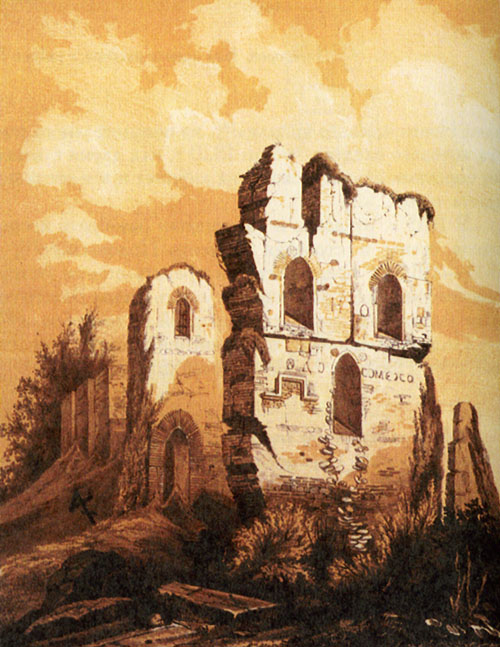
\includegraphics[width=0.82\linewidth]{chast-volga/olga/pannemoker-1826.jpg}

\textit{Вот они. Паннемокер, гравюра 1884 г. с литографии из «Галереи киевских достопамятных видов и древностей» 1864 г., а литография сделана с неизвестного рисунка.}
\end{center}

Вся последующая привязка названия «Десятинная церковь» и этого места основана только на утверждении Могилы. На остатках стен были надписи, до нас дошла перерисовка лишь одной, на непонятном языке, частью греческими и латинскими буквами, и неясно, так ли было или художник неверно передал.

\begin{center}
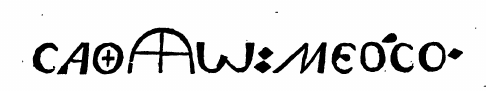
\includegraphics[width=\linewidth]{chast-volga/olga/caption.png}

\textit{Перерисовка надписи со стены этих развалин. Из «Описания Киева» Берлинского.}
\end{center}

Ни при Могиле, ни после, никакого гроба-саркофага с окошком и женскими останками там не обнаружили. В разное время, с 19 века, при раскопках на месте голословной «Десятинной» и около, находили разные каменные гробы-саркофаги, похожие больше на старинные вещевые лари, нежели на те египетские штуки, что возникают в воображении у читателя при слове «саркофаг». Некоторые из этих саркофагов ученые пытались называть гробом Ольги. Из книги в книгу кочует снимок одного такого, за подписью, что это предположительно саркофаг Ольги – а иногда без этой оговорки, утвердительно.

Сей огромный – не «гроб мал» – шиферный саркофаг, без каких-либо признаков окошка, украшенный по бокам крестами вперемежку с листьями папоротника, а на крышке узорами, ныне стоит в трапезной Софии. Подробности его обнаружения в 1909 году освещала газета «Киевлянин».

Будто бы саркофаг сей находили и прежде, о чем писал в своей книге Закревский, сообщавший, что кроме скелета, при раскопках под руководством митрополита Евгения Болховитинова и архитектора Ефимова, в 1826 году, там была обнаружена «истлевшая женская одежда, парчовое покрывало и башмаки». 

Тогда же содержимое саркофага ограбили, сняв драгоценности и сдвинув кости. Вероятно, одежду тоже выкинули, иначе бы в 1909 году не вспоминали написанное Закревским. В статье 1909 года умалчивают, что саркофаг этот нашли вне границ древней якобы «Десятинной» церкви, хотя конечно для версии о том, что это «княгиня Ольга», чей гроб покоился внутри церкви, опущение такой подробности просто необходимо. По одежде тогда определили и пол умершего. 

А вот в 1909 году пол останков вызывал споры. Одни врачи и археологи говорили, в гробнице – скелет женщины преклонных лет. Однако некий доктор Жук утверждал обратное – скелет мужской.

Тогда во время раскопок с гробницей поступили довольно странно. Отыскав оную, оттуда без разбора вынули все кости. Ученые (а где они раньше были?) спохватились позже. В статье А. Савенко (Киевлянин, 24 августа 1909 г., №234), которой считает, что речь идет о саркофаге княгини Ольги, писано: 

\begin{quotation}
Я знаю одного ученого архитектора, который плакал, увидав, что сделали с гробницей. На днях я пошел еще раз посмотреть гробницу и мне стало невыносимо больно: гробница по углам обломана, крышка переломана, а внутри гробницы сидел рабочий и своими толстыми сапожищами топтал место вечного упокоения величайшей русской женщины...
\end{quotation}

Кости вынули вечером, при свечах, и разложили на бумаге. Потом из них составили целый скелет и показывали его в «Десятинной» же церкви. Дальнейшие его перемещения в истории я не смог проследить. Учитывая, что духовенство в 1909 году никак не сообщило об «открытии мощей Ольги», надо думать, что это событие если и не прошло мимо него стороной, то по крайней мере скелет не был признан им, духовенством, за скелет княгини Ольги.

Итак, вне остатков именованной Могилой «Десятинной» церкви, был найден гроб, вовсе не похожий по описанию на тот, в котором лежало тело Ольги. Значит, не там и не такой. В обнаруженном разоренном гробу находился скелет человека невесть какого пола, а также кусочки материи и кожи от обуви. Всё. 

На основании этого сложно делать какие-либо четкие выводы. Трудности определения пола частично льют воду на мельницу моей ереси, что Вещий Олег и Ольга – одна личность. Но, повторюсь – данные слишком скудны, чтобы использовать их в рассуждениях.


О Десятинной церкви. Летописи говорят, что Владимир построил ея на месте дома принесенных их в жертву Варягов-христиан, отца с сыном. Раскопки, однако, показали, что церковь возле Исторического музея была построена на кладбище с многочисленными именно христианскими погребениями, помимо языческих.

Причем христианские захоронения датируются временем начиная примерно за сто лет до княжения Владимира. Хоронили там и после разрушения церкви, а последние могилы относятся к 17 веку. При древнейших покойниках найдены монеты  разных василевсов, например Михаила III (842-867 годы), Василия Македонянина (867-886), однако не позже последнего. Выходит, не только до Владимира, но и до Ольги здесь было кладбище, а окрестности продолжали служить той же цели и после возведения церкви. Саркофаги могли принадлежать кому угодно. 

Учитывая, что при Петре Могиле оставались только развалины здания, кладбище и руины в течении многих лет грабили все, кому ни лень. Могила взял из выкопанного саркофага (где лежали два тела – в отличие от расхожей версии, что нашли два саркофага, Владимира и его жены) голову покойника и руку, и назвал их мощами Владимира. А на саркофаге будто было написано, что тут покоятся Владимир (Василий) и его жена Анна.

По данным же Хроники Титмара Мерзебургского, два саркофага, Владимира и Анны, пребывали в Киеве посередине церкви «мученика Христова папы Климента».

%При Могиле на развалинах стояла деревянная церковь Николы Десятинного. Могила снес ея, возвел новую – Рождества Пресвятой Богородицы, с каменной башней и деревянным притвором. 

На месте раскопанных развалин, Петр Могила возвел церковь Рождества Пресвятой Богородицы, с каменной башней и деревянным притвором. В 19 веке её убрали и поставили ту похожую на дородную купчиху церковь, которую в 1936-м разобрали на кирпичи. 

При устройстве калориферного отопления той последней «Десятинной церкви», в 1905 году, рабочие прокладывали трубы и нашли пустоту, оказавшейся нишей в древней части фундамента. А там – гробница из красного шифера, с грудой костей, где чего только не было, кроме черепа и правой руки. Решили, что это и есть тело, от коего Могила отделил голову. Сей саркофаг стоял в «Десятинной», под спудом, до 1936-го, а что случилось с ним после, я не знаю. След же головы тоже теряется с конца 1930-х.

Но про Ольгу. Казалось бы, говорить уже нечего – умерла, могила ее потеряна, чего же боле?
